In this chapter we describe \demo~\cite{korsveien2014vizpub}, a tool we
propose for visualizing the performance of overlay-based Pub/Sub
Systems. In addition to describing the tool and its system
architecture, we present several visualizations created by the tool. We
also discuss the benefits of using visualizations when studying and
analyzing pub/sub systems, where we share several experiences using the
tool.

We presented a poster and held a live demonstration of \demo{} at the
ACM International Conference of Distributed Event Based Systems (DEBS),
held in Mumbai in May 2014, where it was awarded the price for best
poster and demo. The implementation code of \demo{} is open source, and is
available in a public repository~\footnote{\demo{} is open source and
    hosted at \url{http://github.com/vizpub/vizpub}}. It is our hope that our tool will be
of benefit to the community, and aid in further development and research
of distributed systems.

\section{System Overview}
\label{sec:overview}

To the best of our knowledge, \demo~is the first tool of its kind. The
tool is able to visualize the execution of any given distributed pub/sub
system step by step with respect to a set of performance metrics. Each
node in the system records records relevant data at selected
\emph{reporter intervals} during system execution. Our tool is then able to pull this data to a
single site, and compute various metrics at a system-wide scale. The
collected data from each interval is then collated into a single
\gexf{} file, which is interpreted by Gephi, which enable replay of system
execution offline.

Our tool supports two types of visualizations visualizations, the first is a
visualization of the overlay structure, and how it evolves over time.
The second type of animation is a hop-by-hop visualization of a single
publication message dissemination, where directed edges represent the
message dissemination path. We provide examples of both types of
visualizations later in this chapter.

There are several benefits to using a tool such as \demo. It enables
researchers and developers to gain a deeper insight into the overlay
structure as well as the publication process. It also has major benefits
as an educational tool, as it provides students with an visual
representation of both the structural evolution of the system, as well
as step-by-step animations of publication message disseminations. This
is useful in order to engage students, and facilitate deeper insight
into different pub/sub systems and their dissemination schemes. Such an
insight is also useful in order to identify potential weaknesses or
deployment anomalies of a given pub/sub systems. When developing the
tool, we encountered many scenarios where \demo~demonstrated its
usefulness. For example, when experimenting with PolderCast, we could
immediately verify that tree nodes were disconnected at the RINGS layer,
as seen in Figure~\ref{fig:pold_disc}.  Using our tool, we were able to
verify that this was caused by an artefact in the input workload where
the three nodes had no overlapping interest with any other node in the
system. We were then able to verify that the nodes were connected at the
CYCLON layer. We are not aware of any other tool or framework that would
allow such easy detection and validation of system behaviour.

\begin{figure}[h]
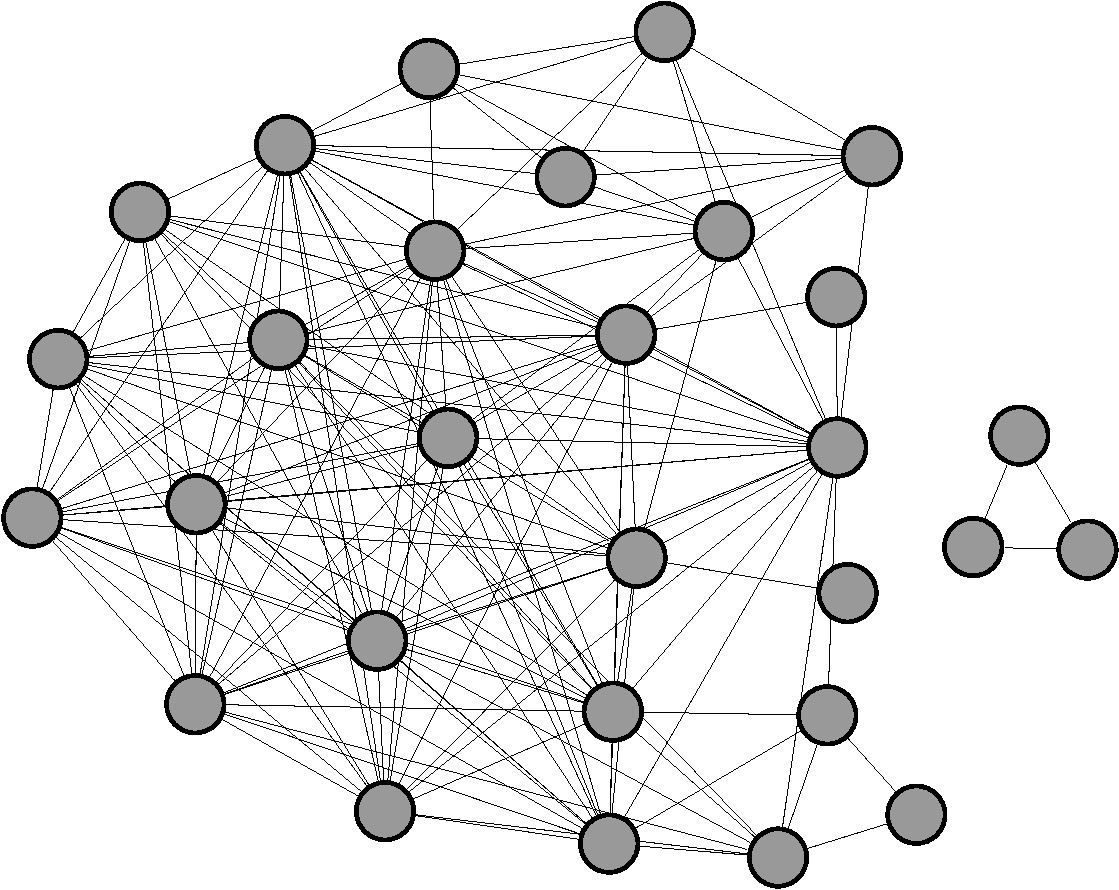
\includegraphics[width=\linewidth]{figures/disconnected-component-poldercast.pdf}
\caption{Visualization of disconnected component in the RINGS layer of PolderCast}
\label{fig:pold_disc}
\end{figure}

Another interesting use case for our tool is comparing different pub/sub systems and
protocols visually. Users may run the different systems using the same
workload, e.g.\ subscriptions and publications, and system parameters in
order to replay the execution and compare the different systems at
selected points in time. We include such comparisons in this chapter,
were we compare PolderCast and Scribe on a set of specific performance
metrics.

\section{Supported Performance Metrics}
\label{sec:metrics}



\section{System Architecture}
\label{sec:arch}

\begin{figure}[h]
\centering
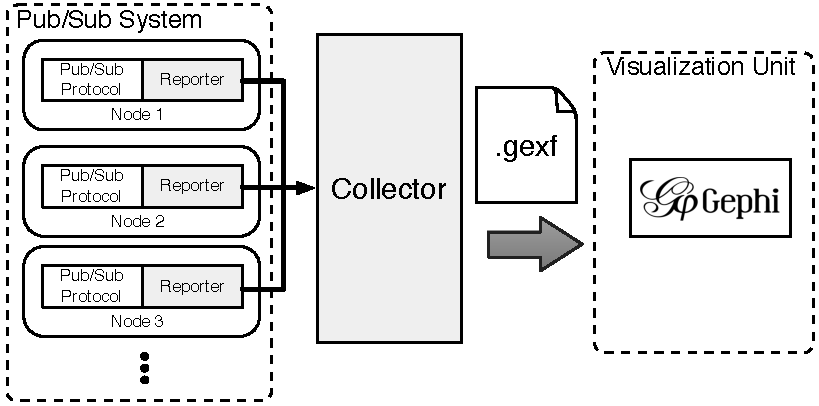
\includegraphics[width=\linewidth]{figures/arch}
\caption{Architecture diagram of \demo}
\label{fig:arch}
\end{figure}

The architecture of \demo~consists of three main components, all
depicted in Figure~\ref{fig:arch}: (1) \emph{Reporter}, (2)
\emph{Collector} and (3) \emph{Visualization Unit}.  The arrows seen in
Figure~\ref{fig:arch} depicts the flow of data in the architecture.
Each node in the executing system consists of a pub/sub protocol as well
as a ``Reporter''. The ``Reporter'' is the entity responsible for
providing the raw information required to compute various performance
metrics from the individual nodes participating in the overlay. This
information is pulled at regular intervals to a central site by the
``Collector'', which translates stores the information as a single
file in the \gexf{} format. This file is then interpreted by the
``Visualization Unit'', which consists of a single machine running
the Gephi tool. The Collector is designed to perform the collection of
data while in online mode, while the computation, aggregation and
derivation of various metrics is performed in in offline mode. The
Visualization Unit always operate in offline mode, as it waits for the
final report to be collated into a \gexf{} format for playback and
visualization.

The design of \demo~supports pub/sub systems that are deployed as
real distributed systems, as well as systems that are deployed in
simulation mode. This is due to the highly modular system architecture,
with strict separation of concerns, where the operation of both the
Collector and the Visualization Unit is separate from the reporting.
\demo~is designed to be a generic tool, where the only system specific
part of the architecture is the \emph{reporter interface} outlined in
Table~\ref{table:interface}. Any researcher or developer
who wants to use our framework only needs to provide an implementation
of this interface, which enables the Collector to retrieve the relevant
data from each individual node at the specified time points. These time
points are configurable, and all the information collected from the
reporter will in effect be the change of the system state from the last
time point with regards to the various performance metrics. We call
these time points \emph{reporting intervals}. The length of the intervals
is configurable, which provides the user with control over the
granularity of data collection, and thus the granularity of the
step-by-step replay of system execution performed in the Visualisation Unit. For example, if
running simulation using PeerNet, the user may determine whether or not
the reporting intervals should encompass several simulation cycles. Or,
in a real distributed pub/sub deployment scenario, the user can
determine the time delay between every reporting interval.


\subsection{Reporter}

The Reporter is responsible of providing the relevant data necessary in
order to calculate the desired performance metrics. In order to do so,
we specify a \emph{reporter interface} which is implemented at each
individual node participating in the pub/sub overlay. This interface
enables each nodes to log certain system parameters using its local
knowledge at each reporting interval. This local information is then pulled
by the Collector at the end of each reporting interval by invoking the
reporter interface. The available method calls and what data each method
returns is described in Table~\ref{table:interface}.

% ../tables/interface.tex
\begin{table}[h]
\centering
\resizebox{\columnwidth}{!}{%
\begin{tabular}{ll}
\toprule
Method Name                                       & Returns\\
\midrule
\tt long reportId()                      & The unique id of this node\\
\tt long[] reportNeighborIds()           & The unique ids of this node's neighbors\\
\tt long[] reportTopics()                & List of topic ids this node subscribes to\\
\tt long reportControlMsgsReceived()     & Number of overlay control messages received\\
\tt long reportControlMsgsSent()         & Number of overlay control messages sent\\
\tt long reportControlBytesReceived()    & Number of overlay control bytes received\\
\tt long reportControlBytesSent()        & Number of overlay control bytes sent\\
\tt PubMessage[] reportPubMsgsReceived() & Reports list of publication messages received\\
\tt PubMessage[] reportPubMsgsSent()     & Reports list of publication messages was sent\\

% \emph{reportDuplicatePubMessages(int topic, int messageId)} :  The number of duplicates received for a specific publication\\
% \hline
\end{tabular}
}%
\caption{Reporter Interface Methods}
\label{table:interface}
\end{table}



It is easy to see how the metrics mentioned in Section~\ref{sec:metrics}
can be derived from the methods listed in Table~\ref{table:interface}.
The structural properties of the overlay such as \emph{degree},
\emph{diameter} and \emph{clustering coefficient} can be derived by
reconstructing the overlay topology. This reconstruction can be achieved
through the two very first methods listed in
Table~\ref{table:interface}, namely \texttt{reportId()} and \texttt{reportNeighborIds()}.
For example, in our reporter interface
implementation for the RINGS layer in PolderCast, each node returns its
own id as well as the ids of both ring neighbors and random neighbors.
After this information is pulled, the Collector is able to derive a
graph structure where it first builds every node reported, and then draw
directed edges between these nodes based on the reported neighbor id
information. What topics each node subscribe to is also useful in order
to derive and visualize metrics such as \emph{Topic Diameter} and \emph{Subscription
    Size}. The Collector is able to pull information regarding topic
subscriptions through the \texttt{reportTopics()} interface method call.
Each node will return a set of topic ids, and the Collector is able to
use this information to attribute topics to each node, as well as edges.
In order to add topics to edges, the Collector simply iterates through
the topic id list of each node, and looks for a neighbor who share a
subscription to the same particular topic. A \emph{topic neighbor}. If a
topic neighbor of a node is found, the topic id is added as an attribute
to the edge connecting them. Applying topic attributes to nodes and
edges, provides the Visualization Unit with the ability to strip away
nodes and edges that does not belong to a particular topic, thereby
enabling calculation of topic diameter.

The dissemination properties of a given pub/sub system such as
\emph{hit ratio}, \emph{path lengths}, and number of duplicate publication
messages received can be derived by having each node provide a list of
publication messages sent and received. In order to calculate these
dissemination metrics, the publication needs to have a particular
structure. This structure is described in Table~\ref{table:structure}.
For example, in order to calculate hit-ratio for a specific topic, we
need to divide the number of subscribers of that topic who actually
received the message with the total number of topic subscribers. We
already know the which nodes subscribe to a particular topic through the
\texttt{reportTopics()} method call, and the list of publication
messages received by a node received can be retrieved through the
\texttt{reportPubMsgsReceived()} method call. Path lengths of a
message being published on a particular topic from a particular node may
be calculated in a similar fashion, as publication messages reported from
different nodes with the same id can be ordered based on their timestamp
values.

The number of duplicate publication messages received and sent by each
node is available through the \texttt{reportControlMsgsReceived()}  and
\texttt{reportControlMsgsReceived()} respectively, while the communication
overhead incurred by control messages in terms of bandwidth consumption can be
derived by the \texttt{reportControlBytesSent()} and
\texttt{reportControlBytesSent()} method calls.

% ../tables/pubmessage.tex
\begin{table}[]
\centering
\resizebox{\columnwidth}{!}{%
\begin{tabular}{ll}
\toprule
Message item           & Description\\
\midrule
\tt long  MsgId            & Unique id of the this message\\
\tt long  TopicId          & Topic id for which this message was generated\\
\tt long  SourceId         & Id of the previous hop node\\
\tt long  DestinationIds[]   & Ids of the next hop nodes\\
\tt long  OriginalSenderId & Node id of the message source\\
\tt long  TimeStamp        & Timestamp of the message sent/received\\
\end{tabular}
}%
\caption{Data Structure of a Publication Message}
\label{table:structure}
\end{table}



The structure of the publication messages outlined in
Table~\ref{table:structure} also allows for visualizing the paths of
publication messages. As, mentioned, this is one of the two types of
visualizations the Collector can output as a \gexf{} file (where the other
type is the overlay structure). In such a visualization the Collector
will look at the topic id of the message, and only include the nodes
interested in the particular topic in the visualization. The Collector
will then iterate through the messages sent and received by each node.
By analyzing the message further, the Collector is able to create
directed edges between the nodes which represent the path of the
publication message. The edges are dynamic, i.e.\ they include a Time
Interval attribute, enabling a step-by-step animation, where edges
appear as the animation is played back in the Visualization Unit,
tracing the path of the publication. This enables researchers,
developers as well as students to analyze publication dissemination
schemes hop-by-hop.

In addition to being able to configure at a chosen reporter interval,
users of this tool may choose to only report partial information. For
example users may choose to only report structural information such as
node ids, or only dissemination specific data such as publication
messages sent and received. This flexibility is useful if only a few
aspects of system performance need analysis.

\subsection{Collector}

The Collector is the component responsible for pulling information from
the nodes at every reporting interval. It is also responsible for
aggregating and calculating certain custom metrics. By custom, we mean
any metric that is not included in the Gephi statistics component. These
metrics are usually related to dissemination and include hit-ratio,
duplicate publication messages received and path lengths. Metrics
related to overlay structure can be calculated in Gephi. These metrics
include degree, clustering coefficient, diameter and centralities. Topic
Diameter however, is a special case. In order to calculate topic
diameter, the graph needs to be filtered down to a subgraph which only
includes nodes and edges for a given topic and calculate the metrics for
every such subgraph. To do this manually using
the Gephi GUI-client would be an time consuming and error-prone task.
Therefore, the Collector  leverages the Gephi Toolkit in order to
automate this task. The collector supports what the Gephi community
refers to as \emph{static} and \emph{dynamic} metrics. This is also
referred to in literature and in~\cite{korsveien2014vizpub} as
\emph{instantaneous} and \emph{aggregated} metrics. In this thesis, we
will refer to them as static and dynamic, in order to be consistent
with the terminology used by the Gephi community. In short, static
metrics pertains to a specific point in time, while dynamic metrics is
based on historical values. The statistics component in Gephi includes
both type of metrics, but dynamic metrics only include degree and
clustering coefficient, while the Collector is able to compute dynamic
metrics for all properties such as centralities, hit-ratio and number of
control messages sent and received.

Aggregation of data is performed by serializing each individual report received
from the reporters into temporary files which are stored on disk. The
collector will then iterate through these files and output a final
report using the \gexf{} file format. While collection is done in online
mode, aggregation is performed in offline mode. The offline aggregation
of data prevents the collector from acting as a bottleneck. Indeed, the
collection and aggregation of data is highly decoupled from the
execution of the pub/sub protocol itself. As an alternative,
the Reporters are also able to log reports locally, and push them to
the collector at the end of pub/sub execution.

The Collector will use the information pulled from the reporters in
order to apply attributes to nodes and edges. These attributes form the
basis of node labels and colors in Gephi. For example, number of
control messages sent is a node attribute which can be represented as a
numeric label on nodes. Also Gephi will inspect all nodes for their
``control messages sent'' attribute value, and determine the maximum and
minimum value. These value form a value range which can be used to color
the nodes on a gradient. For example, the closer a nodes value is to the
maximum, the deeper the color of the node.

Some of the attributes are derived from the reported information, such
as \emph{subscription size}, which is derived from the length of the
collection returned by \texttt{reportTopics()}. What attributes to apply
is configurable. The only edge attributes supported by the Collector is
the topics attribute. This is derived by determining the set of
subscribers of a topic and analyzing the edges between them. If two
nodes have an edge between them, they are topic neighbors. The list of
node attributes supported is far more extensive and includes:

\begin{itemize}
    \item Control messages sent
    \item Control messages received
    \item Control messages sent in kilobytes
    \item Control messages received in kilobytes
    \item List of topics subscribed to
    \item Number of topics subscribed to (i.e.\ \emph{Subscription Size})
    \item Number of duplicate publication messages received
\end{itemize}

These attributes describe data pertaining to individual nodes. However,
the Collector will also calculate data which is global to the entire
graph. For example, the collector is able to calculate the average value
for numeric attributes, such as control messages sent for each interval.
The collector iterates through the interval range, and sums the numeric
attribute value of each node that exists in this interval and divide
this number with the number of existing nodes. The resulting averages
are applied to all nodes as labels, even though they represent a global
value, i.e.\ it is not a value specific to the particular node. This is a
workaround, as Gephi does not support displaying graph attributes.
Currently, the global values calculated by the Collector includes:

\begin{itemize}
    \item Hit-Ratio
    \item Average Number of Control Messages Sent
    \item Average Number of Control Messages Received
    \item Average Number of Control Messages Received in kilobytes
    \item Average Number of Control Messages Received in kilobytes
\end{itemize}

The Collector is also able to calculate average intended for
plotting time series using a tool such as gnuplot, rather than be
applied as a node label. Adding support for
these averages as node attributes is not a priority at this point, but
will be implemented in the near future. We describe the supported
calculations in
Section~\ref{sec:viz_eval}, where we further describe the use case
intended for this feature of \demo.

\subsection{Visualization Unit}

The \emph{Visualization Unit} is a machine running the Gephi Open Graph
Viz tool. This tool is able to interpret the \gexf{} file generated by
the Collector and visualize the execution of the pub/sub system in
question.  Gephi provides a rich GUI-experience where the user may
interact with the graph representation, apply layout algorithms, filter
the graph , execute metrics, apply color and size based on graph
properties and animate the graph evolving over time.  The Gephi software
architecture is highly modular and supports extensions via plugins, some
of which are available in a official plugin
marketplace.\footnote{\url{http://marketplace.gephi.org}}. New metrics,
filters or added functionality such as database support may be
implemented through plugins by developers, and published to the
marketplace free of charge.

Gephi provides many tools and components which are useful when
inspecting and analyzing pub/sub overlays visually. These are what we
consider the most important ones:

\begin{figure}[h]
    \centering
    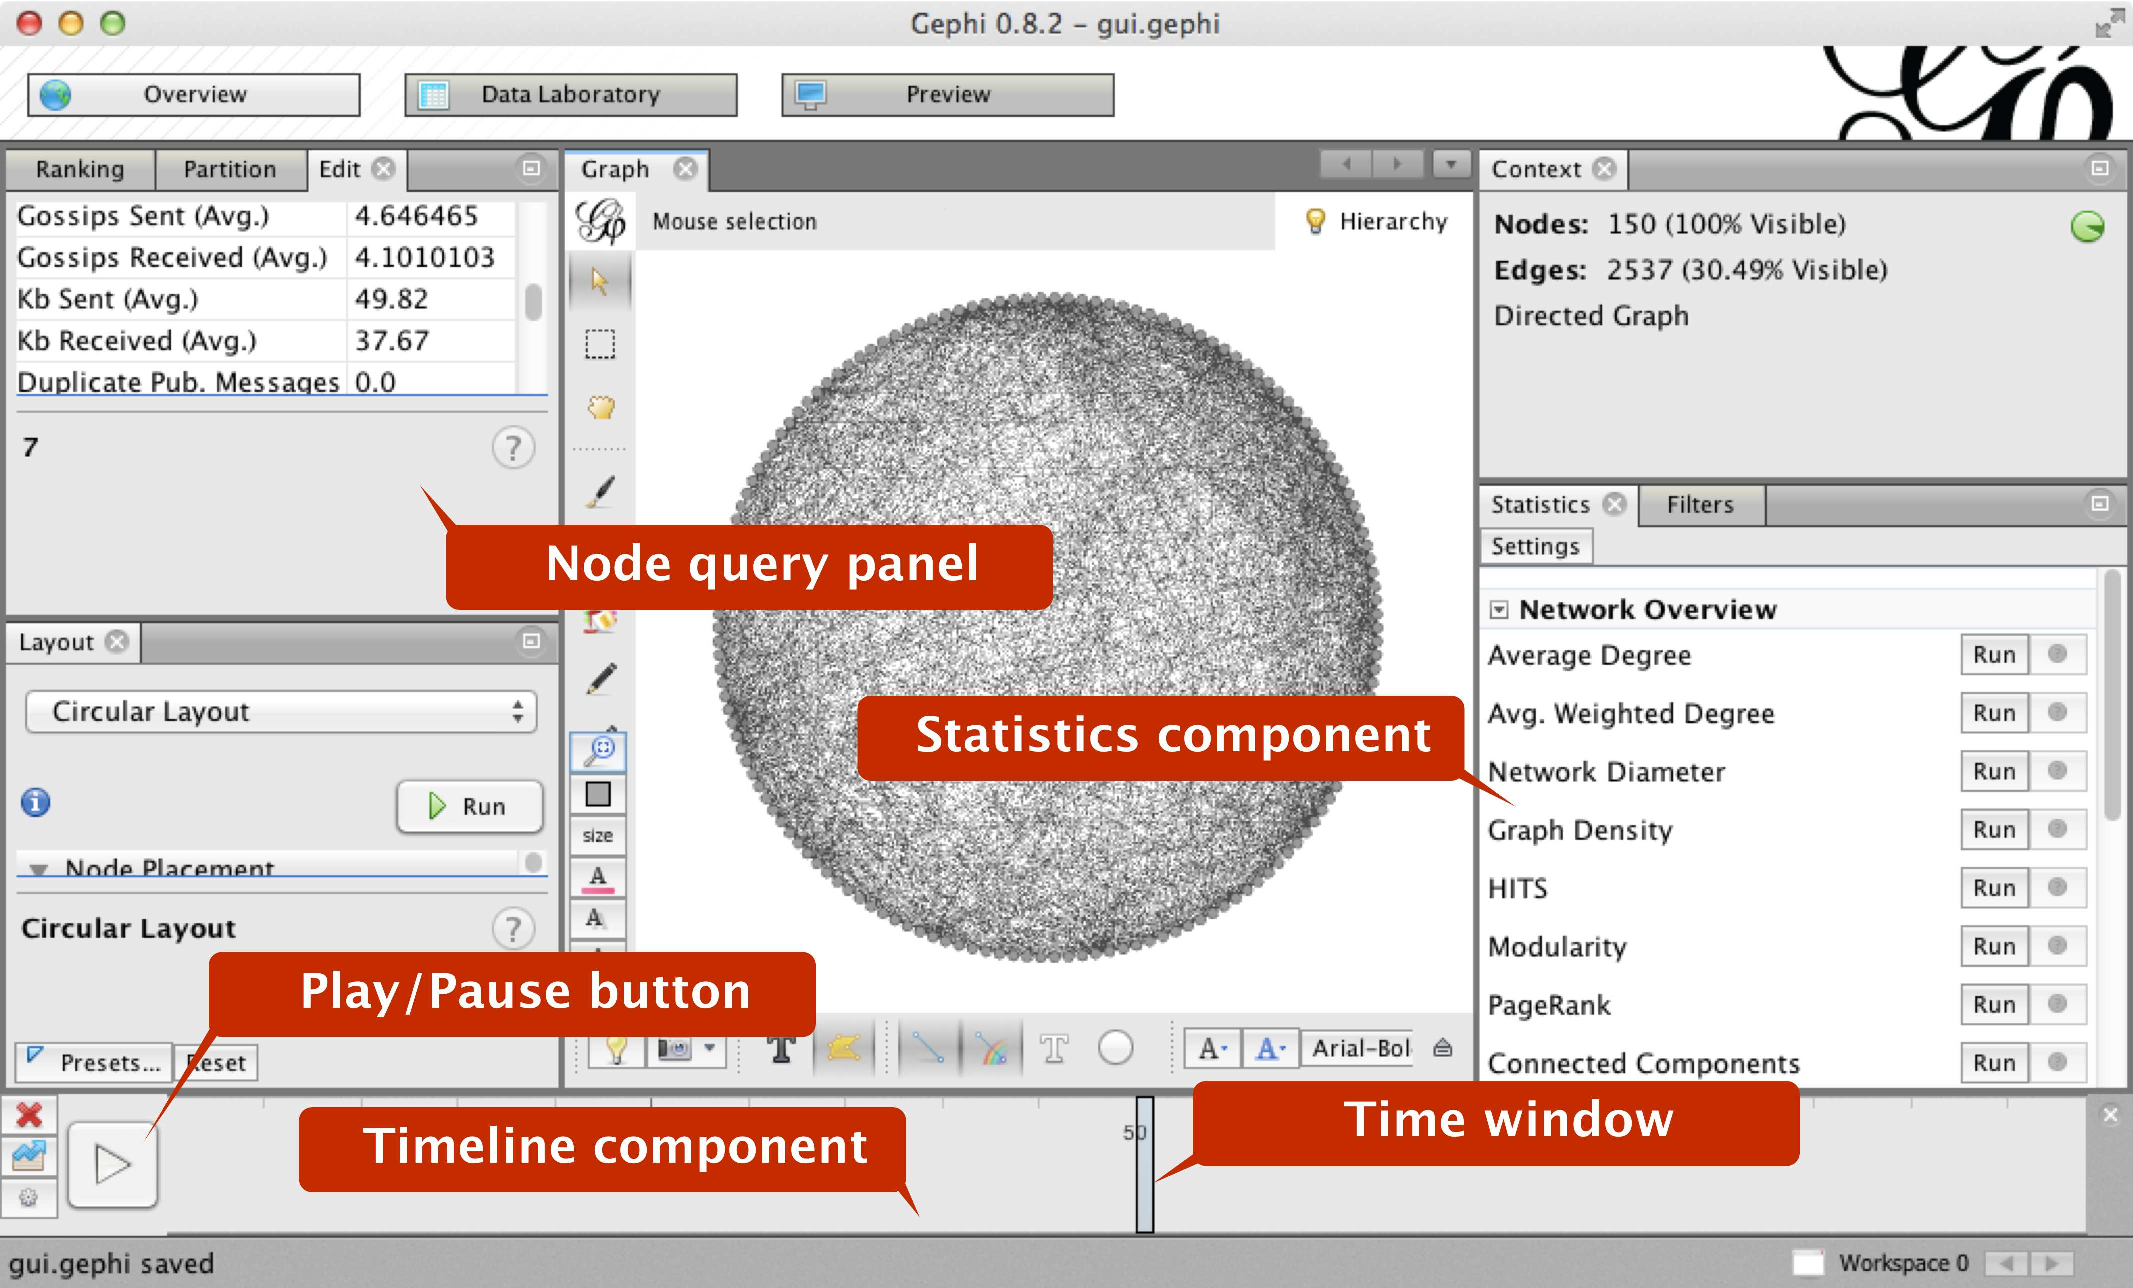
\includegraphics[width=\textwidth]{figures/gui_ann}
    \caption{Snapshot of Gephi GUI with several important components
        annotated}
\end{figure}

\begin{description}

\item[Node Pencil and Edge Pencil Tools] \hfill \\

    These two tools enable the user to create nodes and edges by
    clicking in the graph view, which is the window where the nodes and
    edges are rendered. Edges can be directed or undirected,
    where direction is indicated with an arrow. These two tools combined
    enables building a graph by hand.

    Building such graphs can be useful in order to reason, analyze or
    learn network algorithms such as event dissemination algorithms.
    For example, the user can start with a single node which can act as
    the event source, and build the topology with directed edges which
    depict the path of the message. This is very helpful in fully
    understanding such algorithms and the trade-offs they make. The user
    can also add attributes to the nodes and edges either through the
    \emph{Node Query Tool} or in the \emph{Data Laboratory} component
    which also aids in visualising and understanding properties,
    as well as any drawbacks and advantages of such algorithms.

\item[Node Query Tool] \hfill \\

    \begin{figure}[h!]
        \centering
        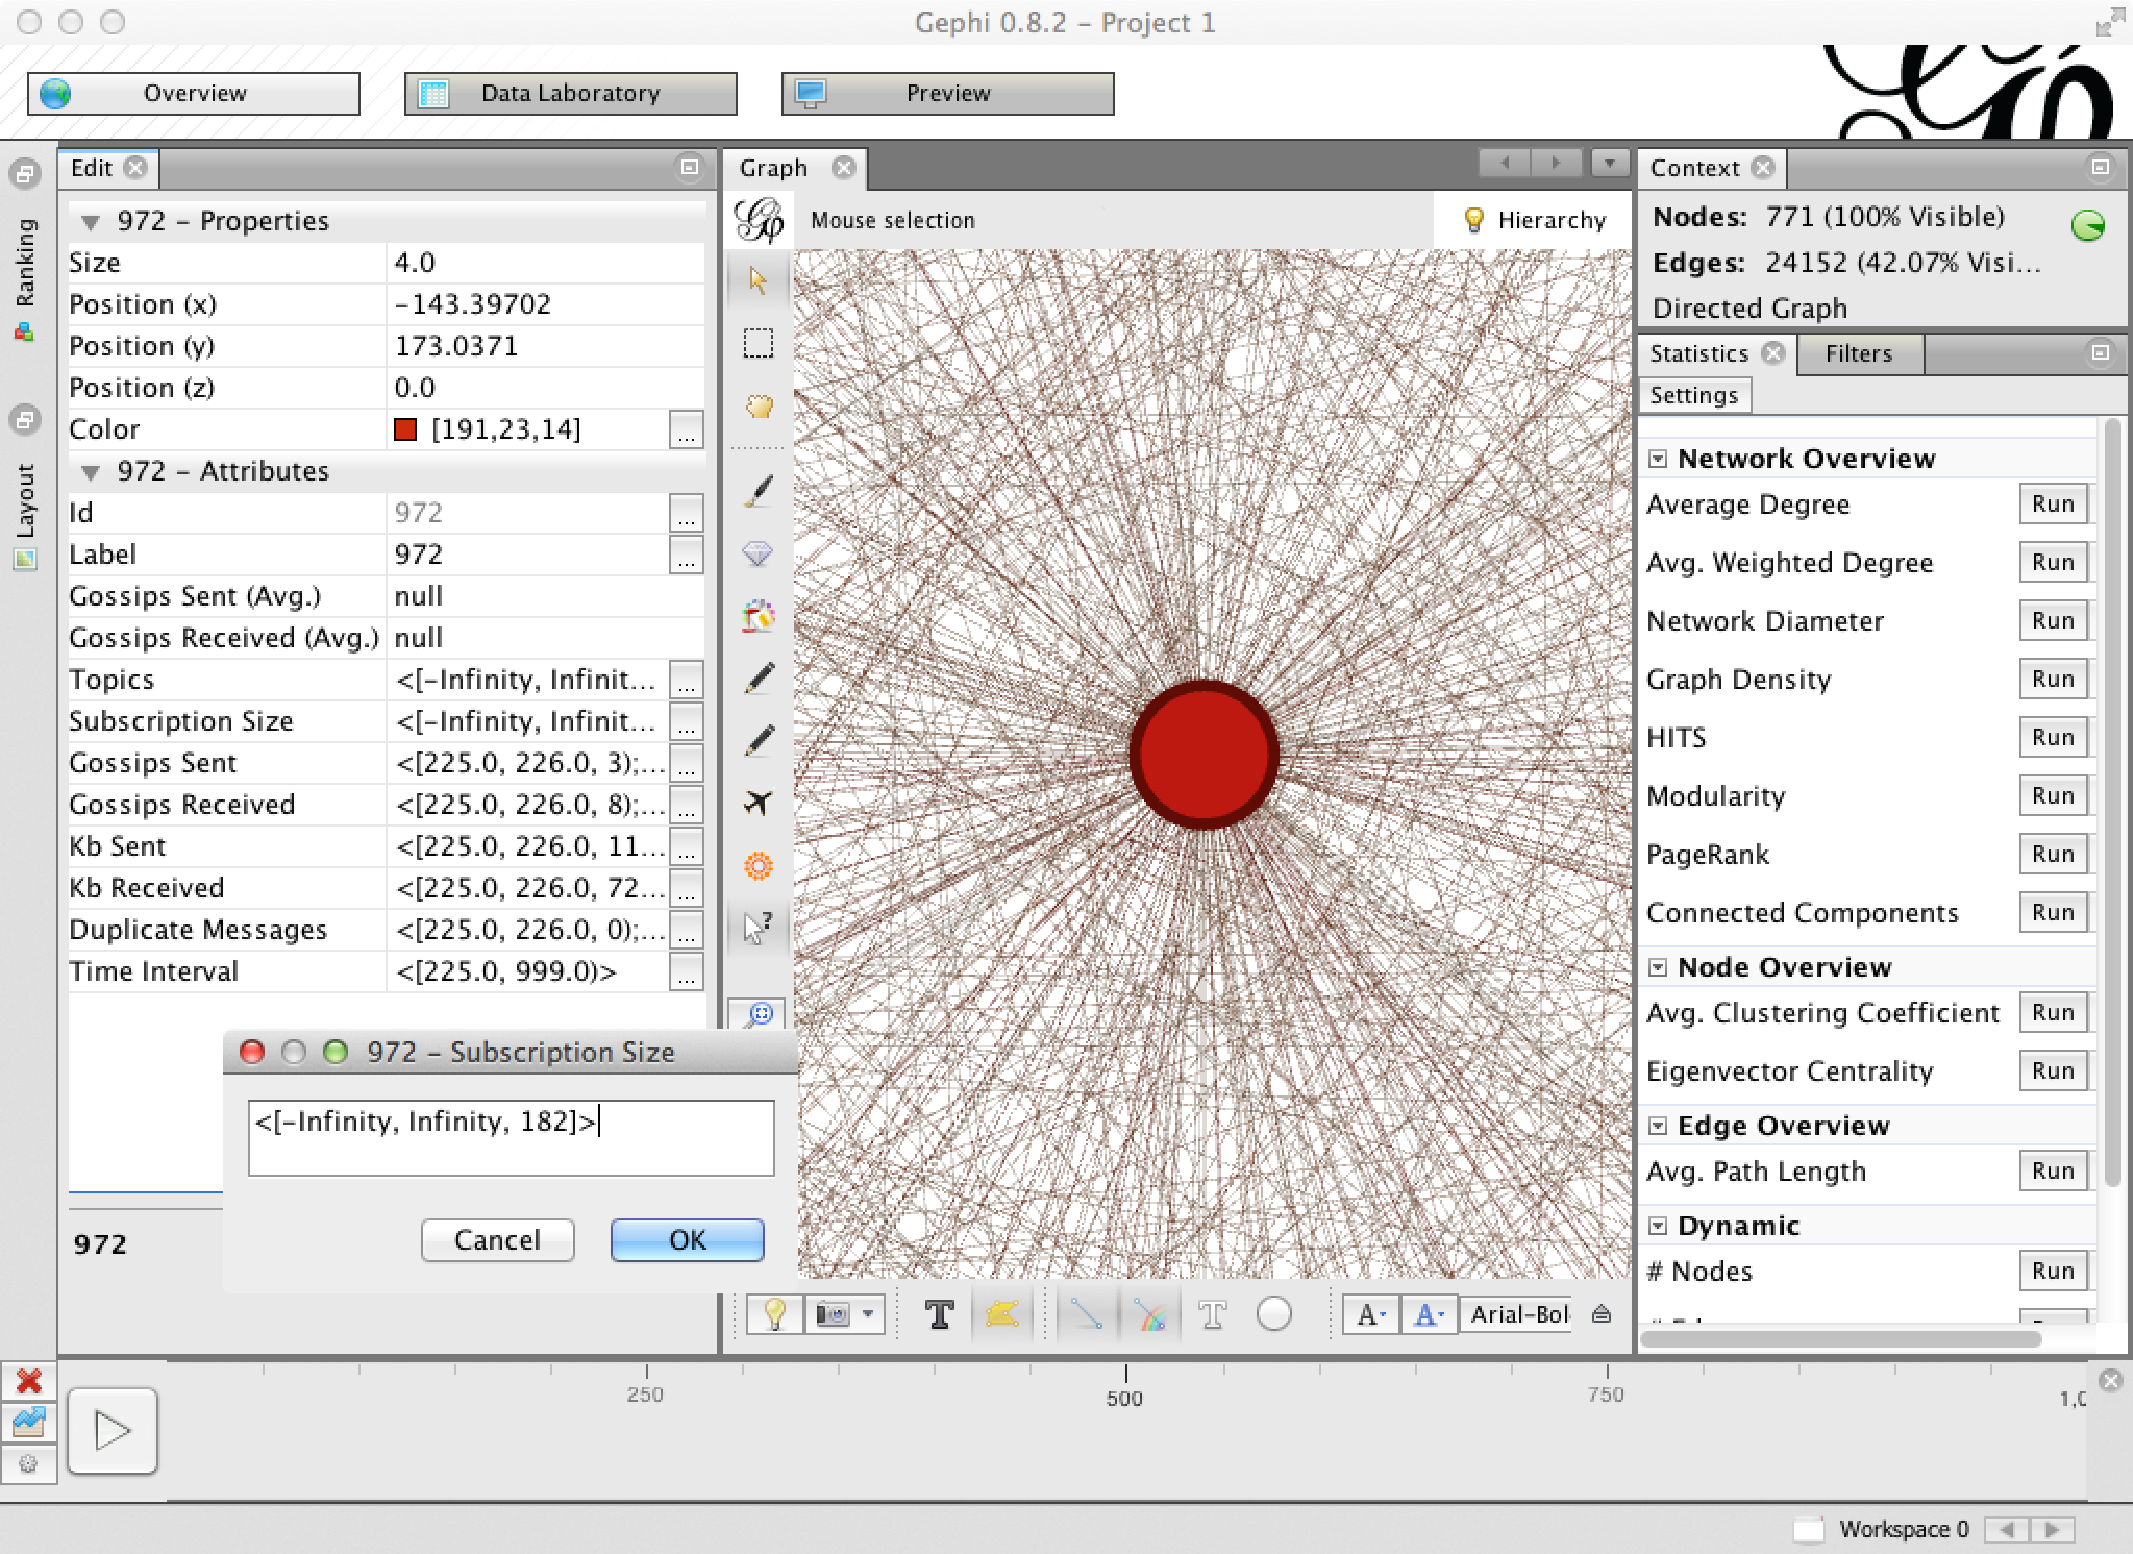
\includegraphics[width=\linewidth]{figures/gui_node_query}
        \caption{The Node Query Tool opens a panel (to the left) that can be used to inspect the
            attributes of a node, here it is used to inspect the
            subscription size of a high-degree node}
        \label{fig:gui_node_query}
    \end{figure}

    With the Node Query Tool the user is able to click on a node in the
    graph view, and a panel will appear to the left with information
    regarding the \emph{properties} and \emph{attributes} of this node.
    Properties are data describing the visual parameters of the node
    such as size, position and color, while attributes include data such
    as node id, default label, the time intervals in which the node
    exists as well as any additional user defined attributes. In our
    case, examples of such user defined attributes would include topics,
    subscription size and number of control messages sent and received.
    The Node Query Tool can be seen in Figure~\ref{fig:gui_node_query},
    where it is used to inspect the \emph{subscription size} (i.e.\ number of
    topics the node subscribes to) of a high-degree node.

    Both the properties and attributes of the node are editable through
    the Node Query Tool. The user may select a property to change the
    visual representation of the node, or select an attribute in order
    to change its value. The \emph{Time Interval} attribute in
    particular is interesting to edit, as it represents the points in
    time in which a node exists in the graph view. For example, it could
    be interesting to edit the Time Interval attribute for certain
    nodes in order to see how it affects a particular metric as well as
    the structure of the overlay topology in general.

\item[Shortest Path Tool] \hfill \\

    With the shortest path tool selected, the user may click on two
    nodes in the graph view, and if there is a shortest path between
    them, this path will be highlighted with a color. This is useful in
    order to reason about the relationship between key nodes in the graph,
    or to compare shortest path between several pairs of nodes.

\item[Heat Map Tool] \hfill \\

    The \emph{Heat Map Tool} enables the user to click on a node in the
    graph view and color its neighborhood based on the edge weight distance between
    them. More specifically, it sets the node color intensity lower for more
    distant nodes and stronger for nodes that are closer. Edge weight is a
    standard edge attribute that is by default set to 1. This means that in
    the default case, the visualization will represent the hop count
    distance from the particular node selected by the user. However, the
    edge weight can be edited by the user in order to represent other
    properties of a system. For example, imagine setting the edge weight
    to represent network latency between two nodes. In this case, a
    neighboring node which is adjacent to the selected node would have a
    lower color intensity if the latency between them is higher than another
    neighboring node which is further away in terms of hop count.

\item[Timeline Component] \hfill \\

    The \emph{Timeline Component} introduces an animation scheme for
    temporal graphs. The user may choose playback parameters such as
    \emph{time interval size}, \emph{step size} and \emph{playback
        speed}. The Timeline will automatically filter out a subgraph
    defined by the upper and lower bound of the interval. The evolution
    of the dynamic graph will then be animated by moving these bounds by
    the distance defined by the step parameter. The delay between each
    step is decided by the playback speed.

    The Timeline enables the user to visually inspect the change in
    graph topology over time, as well as visualize and inspect node and
    edge attributes of the graph through both color, size and text
    labels which is able to change dynamically as part of the graph
    model animation. The Timeline also enables jumping to a specific
    point in time and investigating the corresponding subgraph and its
    properties by changing the upper and lower bound of the Time
    Interval.

\item[Statistics Component] \hfill \\

    \begin{figure}[h!]
        \centering
        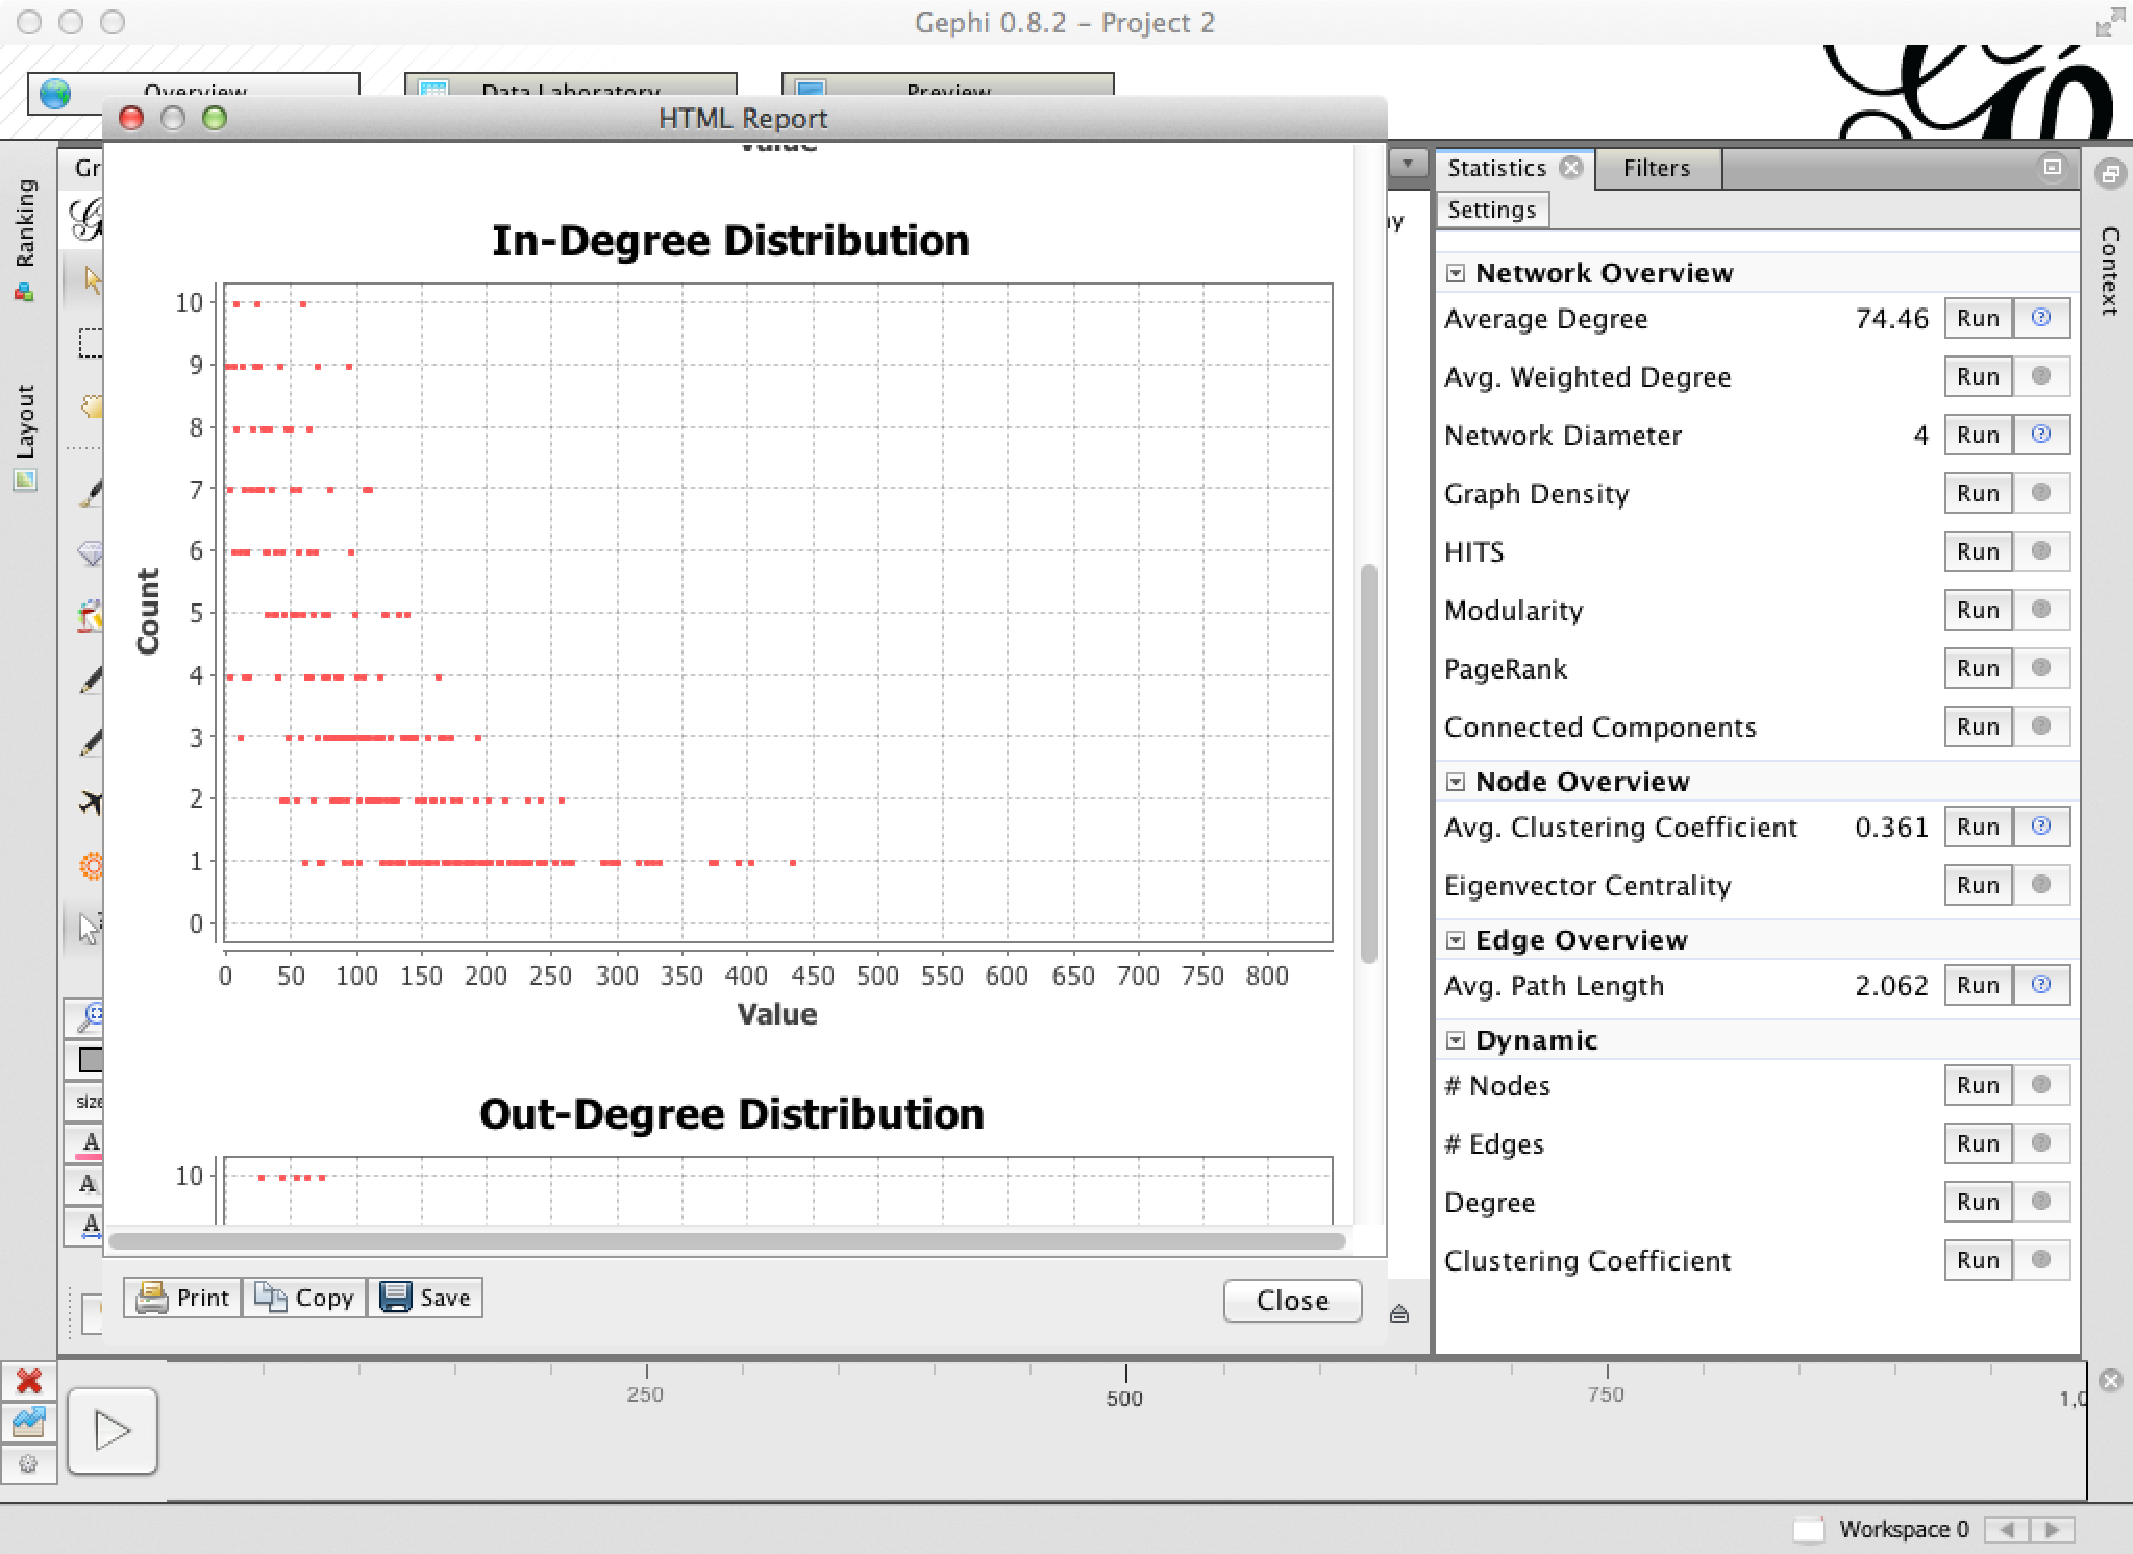
\includegraphics[width=\linewidth]{figures/gui_statistics}
        \caption{The Statistics component is able to produce a HTML
            report which includes plots describing the distribution of
            values across the nodes}
        \label{fig:gui_statistics}
    \end{figure}

    The \emph{Statistics Component} enables graph topology analysis by
    executing metrics on the graph. There are two types of metric
    algorithms in Gephi: \emph{static} and \emph{dynamic}, where the
    former calculates a single value based on the currently defined time
    window, while the latter calculates a time series of values. When
    executing a dynamic metric, the user must define the time window
    size and tick. These parameters have the same functionality as the step parameter
    when using the \emph{Timeline Component}. When the metric executes, the
    time window will iterate through the entire time range of the
    simulation, calculating a value at each step. When finished,
    a time series is plotted and displayed for the user. Such reports
    are also generated and displayed when calculating static metrics. In
    the case of static metrics, scatter plots depicting the distribution
    of values are displayed, as seen in Figure~\ref{fig:gui_statistics}

    The Statistics component include several metrics which are relevant
    to pub/sub overlays. Useful static metrics include, but are not
    limited to:

    \begin{itemize}
        \item{Degree (In/Out/Avg./Max/Min/Distr.)}
        \item{Avg. Cluster Coefficient}
        \item{Centrality (Beetweeness/Closeness/Eccentricity)}
        \item{Average Path length}
        \item{Radius}
        \item{Network Diameter}
        \item{Number of Shortest Paths}
    \end{itemize}

    Out of these, only degree and the clustering coefficient metrics have dynamic
    versions, where both calculates the average value over time. The
    average for dynamic metrics are calculated by dividing the sum of
    all node attribute values with the total number of nodes in both
    cases.

\item[Ranking Component] \hfill \\

    \begin{figure}[h!]
        \centering
        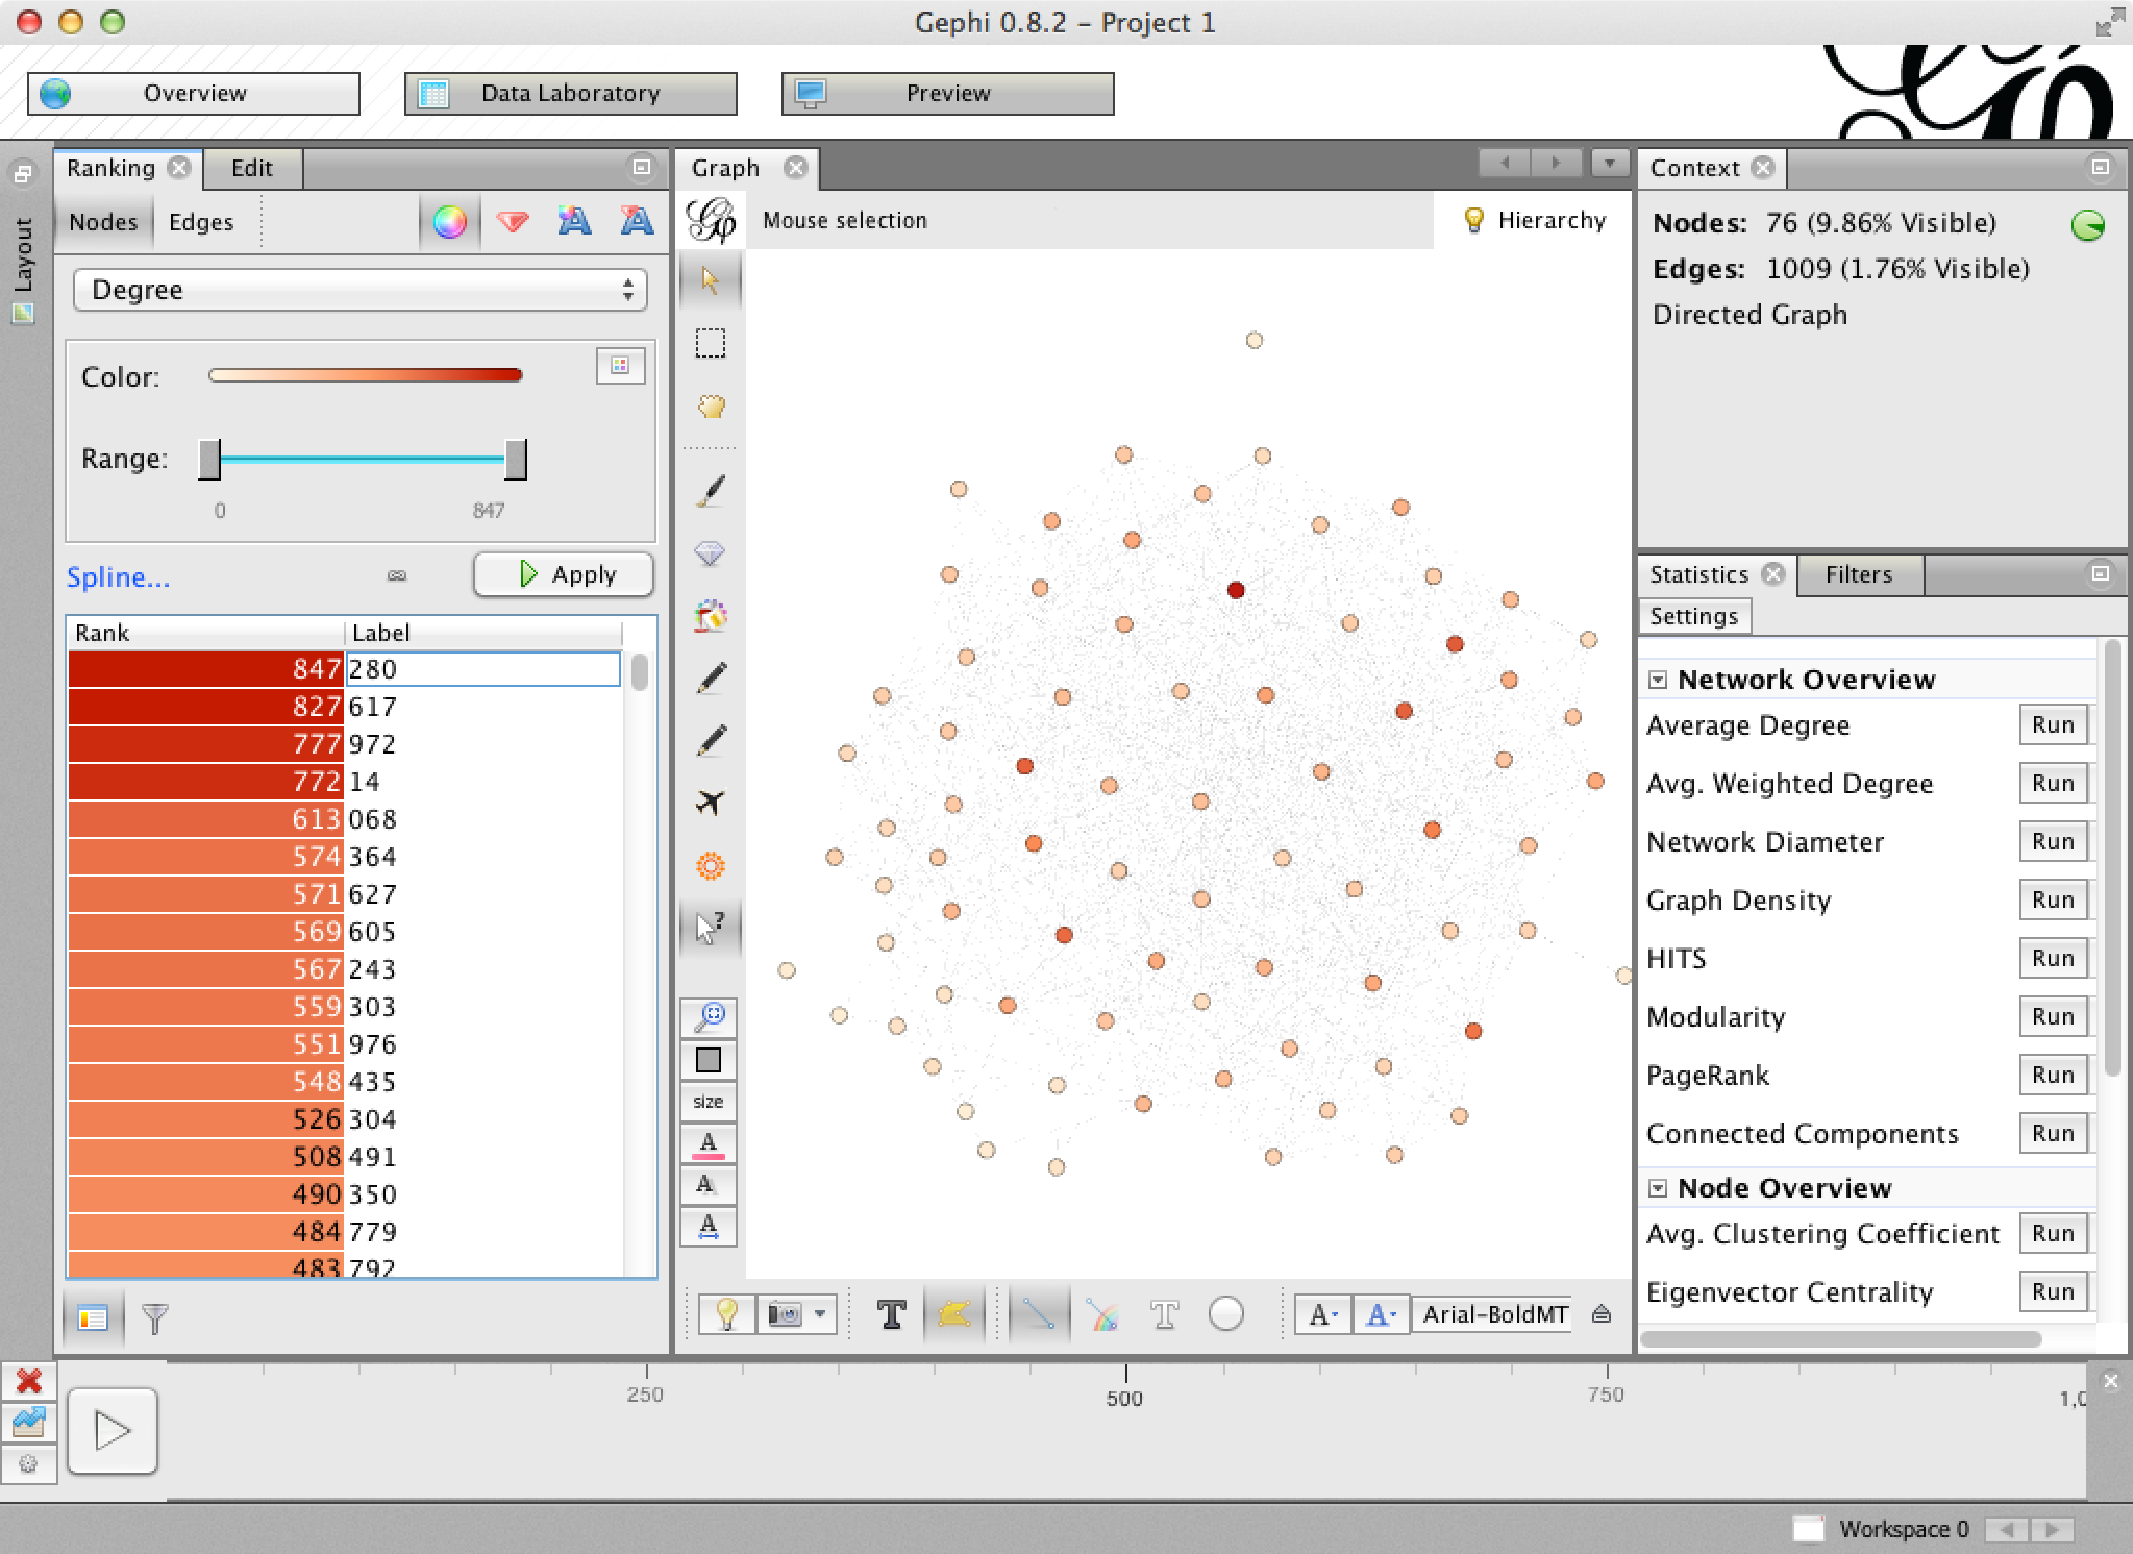
\includegraphics[width=\linewidth]{figures/gui_ranking_table}
        \caption{The \emph{Ranking Table} (to the left) in the Ranking Component may
            be used to sort nodes by attribute value. In this
            screenshot it is used to rank nodes by degree in descending
            order.}
        \label{fig:ranking_table}
    \end{figure}

    The \emph{Ranking Component} is a key feature of Gephi which enables
    visualization based on node or edge attributes in form of color and
    size. When coloring nodes or edges, the ranking component will apply
    a gradient over the range of attribute values. The ranking component
    also include a ranking table, as seen in
    Figure~\ref{fig:ranking_table}, where the user may sort nodes based
    on the specified attribute value. This is useful for quickly finding
    the nodes with maximum and minimum value, which is a quick way of
    identifying bottlenecks in the system or potential load balancing
    issues.

    The Ranking Component also includes an auto apply feature, which
    supports visualising attributes dynamically while playing back the
    graph via the \emph{Timeline Component}. More specifically, the node labels and color
    will update with every step of the animation.

\item[Layout Component] \hfill \\

    The \emph{Layout Component} enables the user to execute algorithms that
    calculates the position of the nodes. The user is able to adjust the
    parameters of these algorithms in order to manipulate the visual
    layout. The different algorithms emphasize different aspects of the
    topology. One example is the so-named \emph{Force Atlas} layout algorithm which
    simulates the effect of gravity on the nodes, where linked nodes
    attract each other and non-linked nodes are pushed apart. This
    particular algorithm is useful for visually detecting clusters and
    communities. Another useful algorithm is the \emph{Circular Layout}
    algorithm, where nodes are positioned in a circle ordered on a
    specific node attribute selectable by the user. This is useful in order
    to visualize node rankings on particular attributes. We use the
    circular layout extensively, as nodes in PolderCast are organized
    into a ring structure, where they are ordered by their unique id.

\item[Filter Component] \hfill \\

    \begin{figure}[h!]
        \centering
        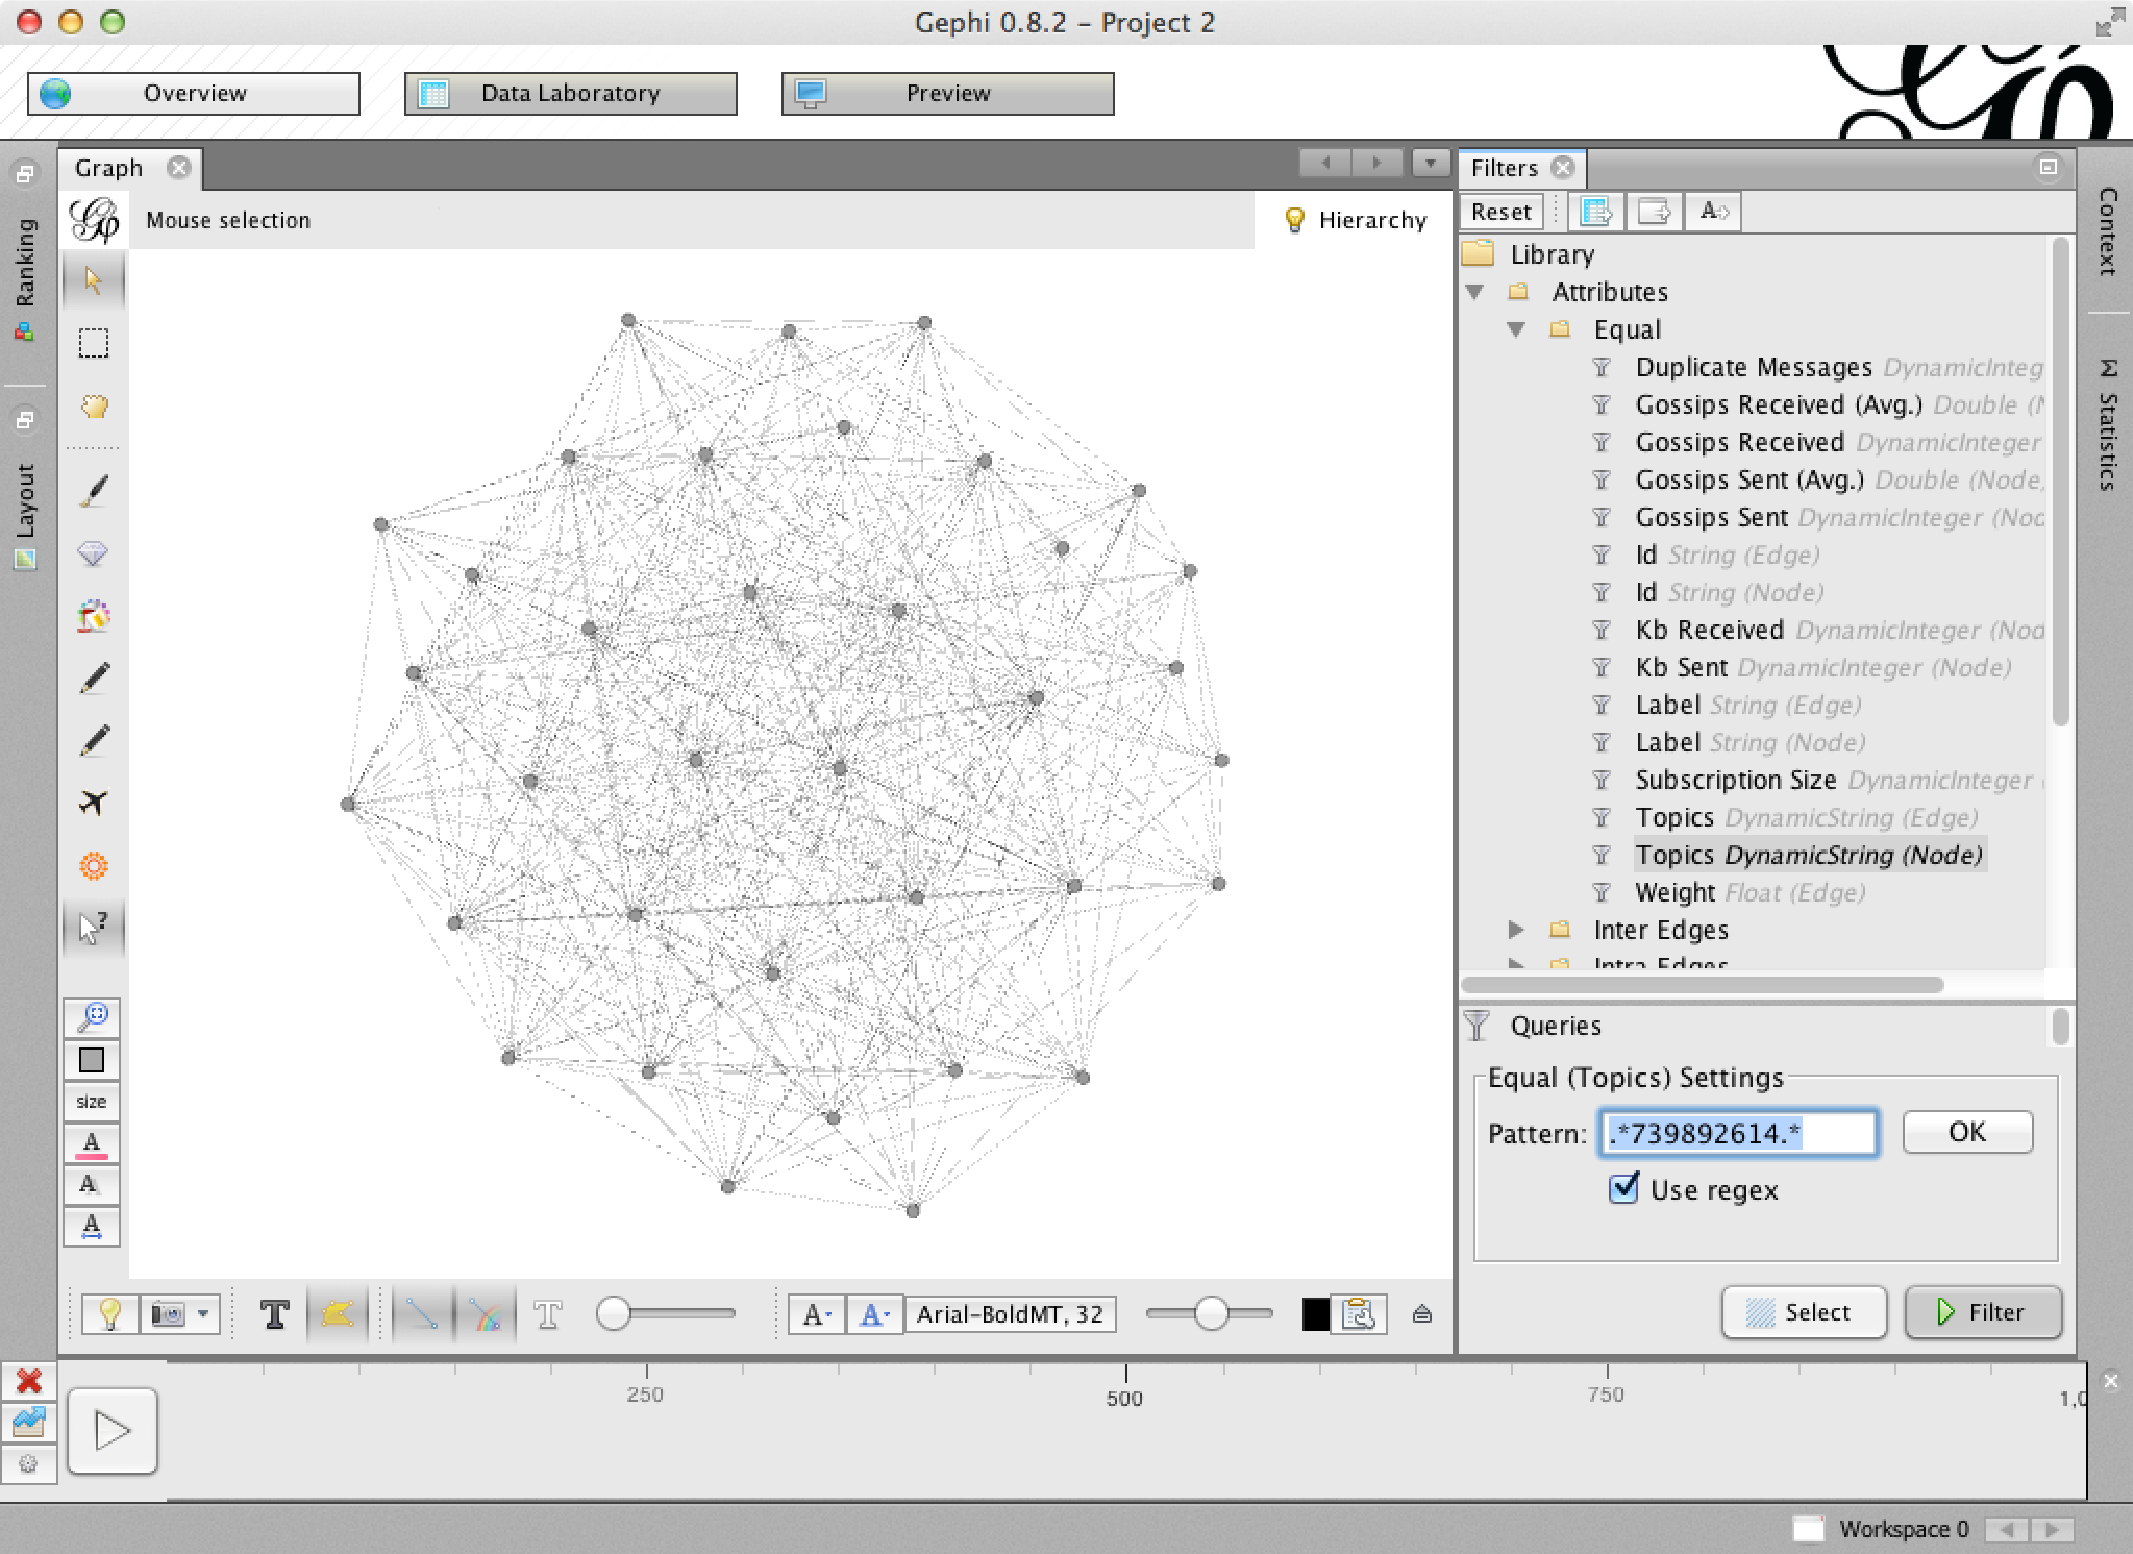
\includegraphics[width=\linewidth]{figures/gui_filter}
        \caption{The Filter Component (to the right) enables users to strip away
            unwanted nodes and edges, in this screenshot it is used to
            display the sub-overlay for a specific topic by using a
            \emph{regular expression}.}
        \label{fig:ranking_table}
    \end{figure}

    \emph{Filters} may be applied to the graph in order to strip away
    nodes or edges on the basis of their attributes. Filters may strip
    away nodes based on a value range if the attribute type is a number,
    or they can be matched on a regular expression if the attribute is
    encoded as a string. Filters can also be combined through special
    operator filters representing set operations such as union and
    intersect.

    Filters are an essential mechanism in order to analyze subgraphs.
    For example, in order to calculate \emph{topic diameter} in pub/sub systems,
    a subgraph can be filtered out based on a \emph{topic attribute}. Then, the
    diameter metric can be executed on this subgraph, which will result
    in the diameter of the particular topic.

\item[Data Laboratory Component] \hfill \\

    \begin{figure}[h!]
        \centering
        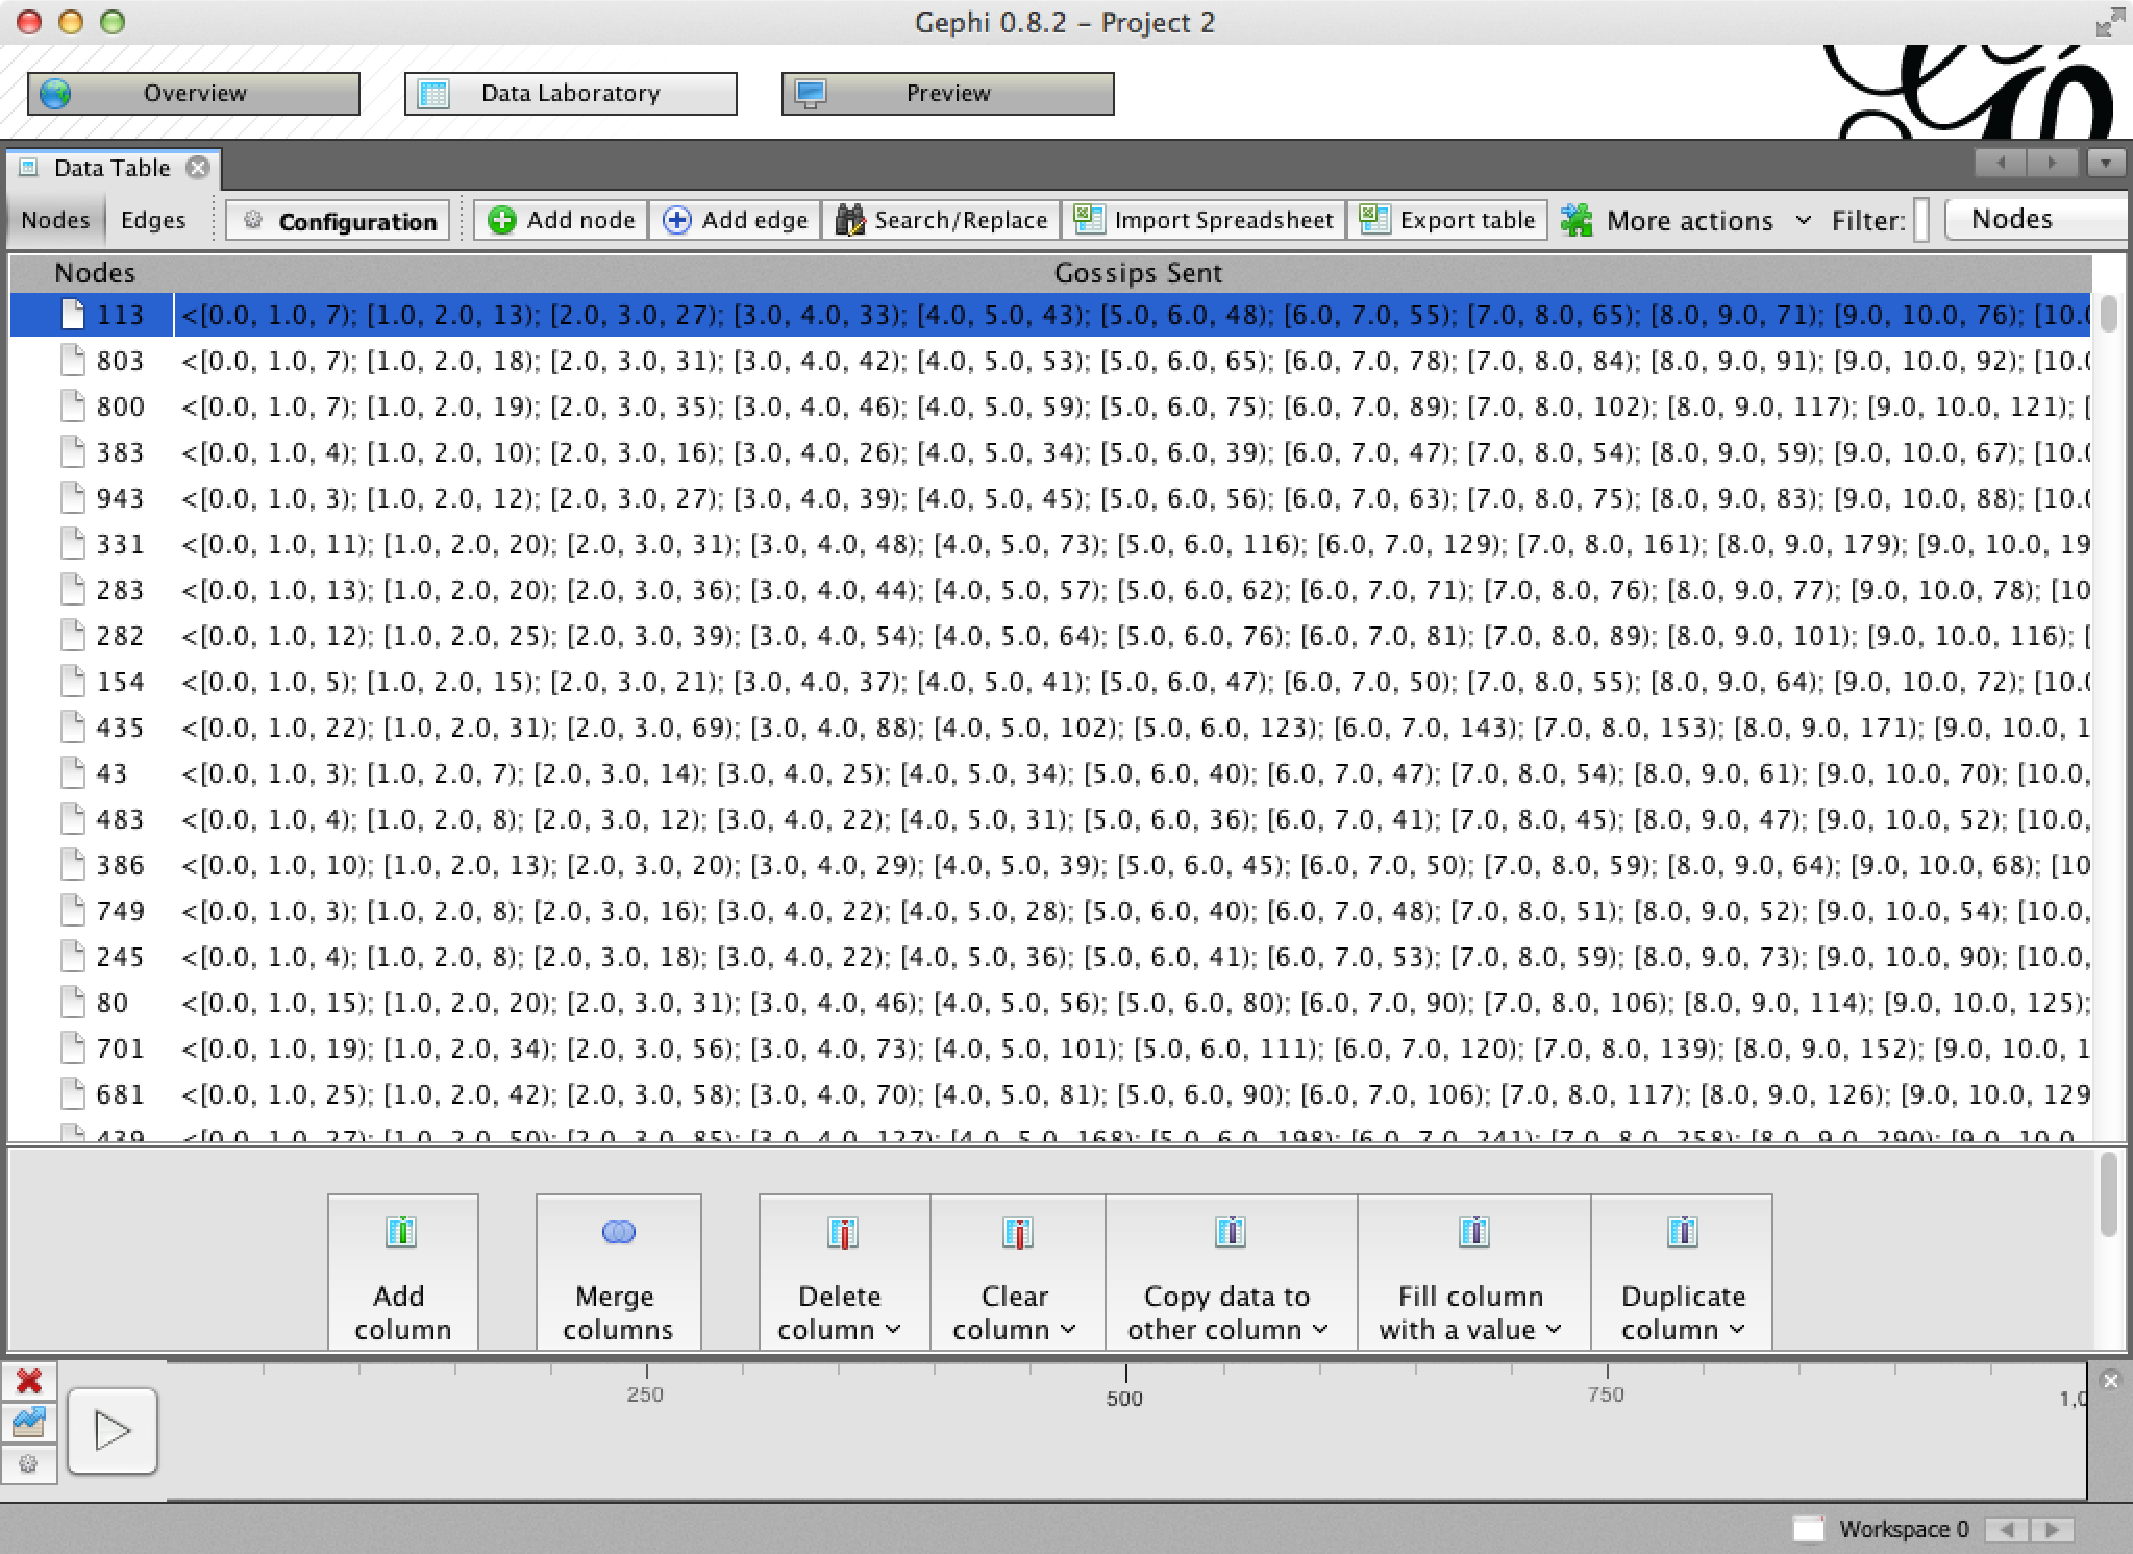
\includegraphics[width=\linewidth]{figures/gui_data_lab}
        \caption{The Data Laboratory Component provides a table overview
        of metrics as well as the capability of exporting data.}
        \label{fig:data_lab}
    \end{figure}

    The \emph{Data Laboratory Component} enables the user to work with
    the node and edge attributes of the graph. This component provides
    the user with separate table views of node and edge attributes, as
    seen in Figure~\ref{fig:data_lab}. Each row in this table represent
    a node or edge, and each column an attribute. Columns may be added
    or removed by the user. The Data Laboratory also provides
    functionality for manipulating columns such as merging two columns
    or creating new columns based on the data from selected columns.
    Attribute data in columns that are static (i.e.\ has no lower or
    upper time interval bound associated with them) can be converted to
    dynamic through this component. Also, resizing or coloring all edges
    or nodes is possible through the laboratory by selecting all rows
    and right-clicking. In addition to this, the Data Laboratory also
    enables the user to export the data to file for further statistical
    analysis.

\end{description}

\section{Examples of Visualizations}

In this section, we present a number of visualization produced by \demo.
The examples we provide in this section include both visualizations of
overlay structure as well as hop-by-hop message dissemination.  We
implement a reporter interface both for PolderCast as well as Scribe and
provide examples of visualizations for both protocols and compare them
visually on various performance metrics. Both protocols are implemented
using the PeerNet P2P simulator by updating existing PeerSim
implementations of Scribe and PolderCast.

Many of these visualizations were part of our demonstration at
DEBS 2014, and should provide some insight the benefits of using
our tool, and what sort of possibilities there are in terms of
visualizing overlays.

\subsection{Data Traces Used in Simulations}

We use publicly available datasets from
Facebook\cite{facebook-eurosys09} and Twitter\cite{Kwak10www}. The Facebook
dataset consists of 3 million user profiles along with 28.3 million
social relations between these users. The Twitter dataset consists of
41.7 million distinct user profiles and 1.47 billion follow/followed
relations. In both datasets users are modeled as topics. In the Facebook
dataset, subscriptions are modeled after the friend list of that user.
As relationships are bidirectional, two topics will subscribe to each
other. In Twitter, relationships are unidirectional, as users may choose
to follow other users, and no user who is followed need to reciprocate.
As a user is modeled as a topic, its list of followers are modeled as
the subscribers of that topic. The simulations we run in this chapter
consists of 2000 nodes, where the workloads have been extracted in~\cite{Setty:2012}.

Churn is based on the Skype super-peer network data
trace~\cite{Guha:2006}, where 4000 nodes are tracked for joining and
leaving timestamps for one month staring on September 12, 2005. Finally,
we use the King dataset~\cite{king} in order to model latency between
nodes.

\subsection{Overlay Evolution During Churn}
\label{sec:churn}

\begin{figure*}[h]
    \centering
    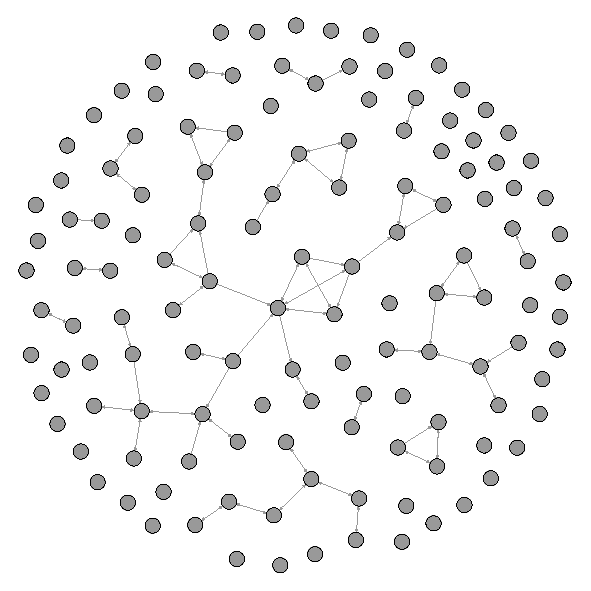
\includegraphics[scale=0.35]{figures/churn_0}
    \caption{Overlay structure of PolderCast at interval 0}
    \label{fig:churn0}
    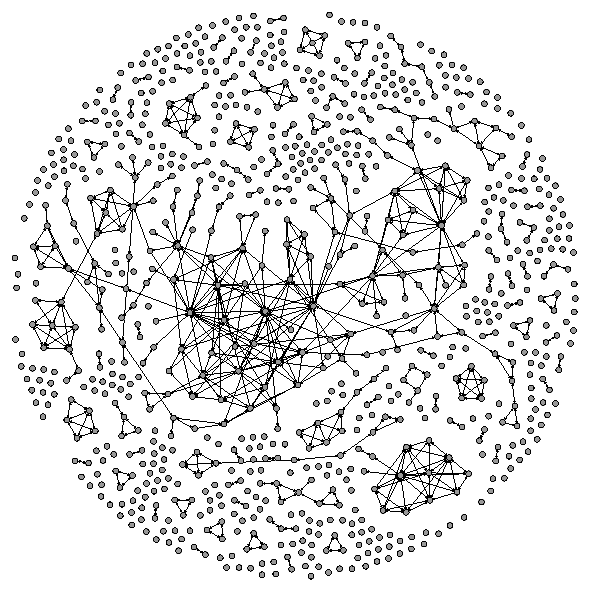
\includegraphics[scale=0.85]{figures/churn_250}
    \caption{Overlay structure  of PolderCast at interval 250}
    \label{fig:churn250}
    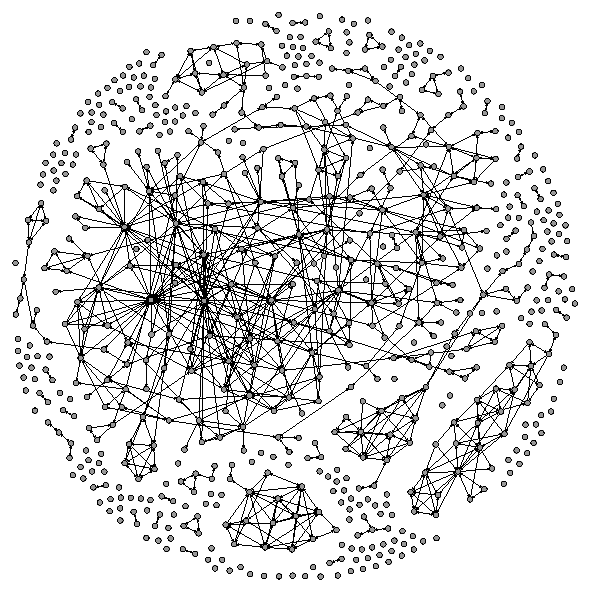
\includegraphics[scale=0.85]{figures/churn_500}
    \caption{Overlay structure of PolderCast at interval 500}
    \label{fig:churn500}
\end{figure*}

In Figure~\ref{fig:churn0},~\ref{fig:churn250} and~\ref{fig:churn500} we
visualize the overlay topology of 2000 PolderCast nodes during churn.
This is one of the examples of visualizations we presented at DEBS 2014.
Each figure corresponds to a reporter interval. Figure~\ref{fig:churn0}
depicts the overlay at interval 0, where 132 nodes are up while the
remaining 1868 are down due to churn. The snapshot in
Figure~\ref{fig:churn250} depicts the overlay at interval 250, after a
considerable number of nodes have joined the network. More specifically,
interval 250 consists of 1028 nodes, which means 896 nodes joined in the
interim. The edges are also evolving. While the first interval consisted
of 108 edges, interval 250 consists of 1028 edges. It is interesting to
see the edges evolve over time, as they provide can provide us with
immediate visual feedback on properties such as clustering of nodes,
graph density and node degree. Such properties can then be further
analyzed using the Statistics component in Gephi.

Furthermore, such visualizations might provide immediate information
regarding the dataset being used. As mentioned in
Section~\ref{sec:overview}, we encountered a scenario where an artefact
in the dataset resulted in a disconnected component in the visualized
overlay. Here we notice that many of the nodes are disconnected. This is
due to a sampling bias, as the Facebook dataset contains 10,000 nodes
while the simulation runs 2000 nodes. However, visualizations including
such a high number of nodes is not appropriate for print due to space
restrictions.

\subsection{Visualizing Performance Metrics}

\demo{} supports visualizing a number of performance metrics. These
metrics are applied as attributes both to nodes and to labels. Here we
will take advantage of these capabilities and present a range of
visualizations for PolderCast, in order to determine what we can learn
from them.

\subsection{Publication Message Dissemination}
\label{sec:dissviz}

\begin{figure}
    \vspace{-100pt}
    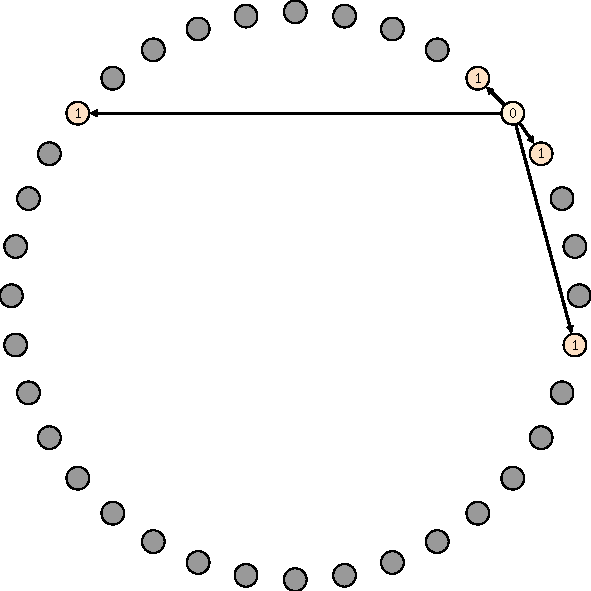
\includegraphics[scale=0.6]{figures/diss_1}
    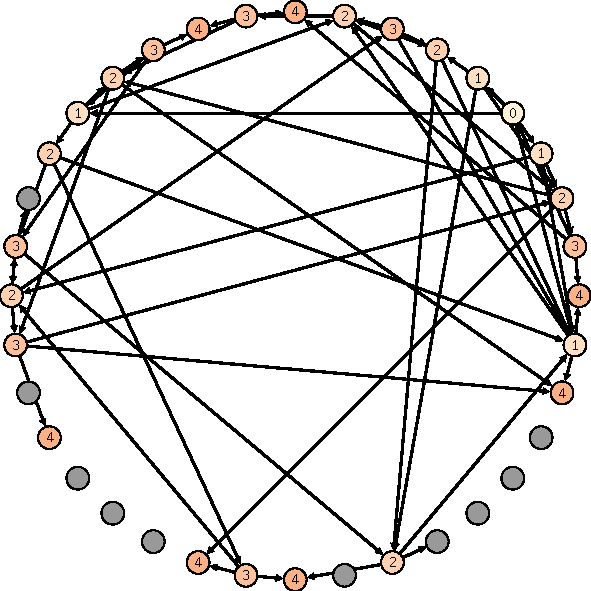
\includegraphics[scale=0.6]{figures/diss_2}
    \caption{From top to bottom: visualization of publication message
        dissemination in PolderCast after 1 and 4 hops.}
    \label{fig:diss_1}
\end{figure}

In subsection~\ref{sec:churn} we illustrate one of the two types of
visualizations it is possible to produce by leveraging \demo. Here we will describe the second:
event dissemination visualizations.

We run a PeerNet simulation in distributed mode with 100 nodes running
the PolderCast protocol with a fanout set to $f=2$. In order to scale
the experiment, the simulation includes 10 machines, where each machine
is running 100 PeerNet nodes.  We publish a single message on the
most popular topic which includes 63 subscribers. By analyzing copies of
the publication message received on each node, the Collector is able to
create a step-by-step visualization where directed edges are drawn as
the message is disseminated through the overlay.  These edges depict the
path of the message being disseminated. The visualization includes 189
edges in total, which indicates how many publication messages was sent
by all nodes during the simulation.

Figure~\ref{fig:diss_1} is a visualization of the dissemination in
PolderCast after 1 and 4 hops, while~\ref{fig:diss_2} are snapshots of
the dissemination visualization after the dissemination has finished.
The nodes have been arranged in a ring using the Layout component in
Gephi. Also they are ordered by node id, making it easier to see whether
an edge represent a ring link or a random link. The labels indicate the
hop number of the message received by that node. On the left side of the
ring there is a node with the label ``0'', which indicates that this is
the publishing node. A node with the label ``1'', means the node
received a message at the first hop, a node with a label ``2'' that it
received a message at the second hop, and so on. In addition to numeric
labels, the nodes are color coded on a gradient. The deeper the color of
the node, the higher the hop count, which means it is further away from
the publisher. In figure~\ref{fig:diss_2} the node furthest away is
easily spotted on the left by its deep red color. This is the last node
to receive the publication.

It might seem strange that the last node to receive the message is an
immediate ring neighbor of a node who received the message on the first
hop. Observe that in Figure~\ref{fig:diss_1} this neighboring node who
received a message on the first hop does indeed send a message to the
node in question. However, in Figure~\ref{fig:diss_2}, which depict the
dissemination after the message has been sent, no numeric label is
applied to the node. This could bear the impression that this note did
not receive any message, however this is not the case. The explanation
behind this is latency. The latency between these two nodes is so high
that by the time it received the message from its ring neighbor, the
message was already received from somewhere else. We choose to visualize
this by drawing an edge to the node and then refrain from applying a
numeric label. When we reach the point in the animation where this node
receives a message for the first time, we apply the hop count of this
message as a numeric node label.

When inspecting the dissemination algorithm of protocols visually,
implementation details which could otherwise be overlooked become easily
detectable. For example, in Figure~\ref{fig:diss_1} it can be observed
that the publisher node sends a message to four nodes, even though the
fanout is set to $f=2$.  This fanout should indicate that the node
should send the message to three neighbors, based on the description of
the dissemination algorithm of PolderCast, summarized in
Chapter~\ref{ch:background}.  However, there is an implementation detail
in PolderCast that is not mentioned in the original
paper~\cite{Setty:2012}. In the implementation of the PolderCast
protocol, publishers send messages to one additional random node in
order to boost the initial phase of the dissemination. Learning such
implementation details is useful to both researchers and developers, and
it is especially useful for students. We believe \demo can be very
valuable as an educational tool, as its grant students with the
capability of controlling the dissemination by using the Timeline
component in Gephi. Students may pause the visualization at any point in
time or jump to any step of the visualization in order to fully
understand the benefits and drawbacks of the particular dissemination
scheme being studied.

It is also useful to create such visualizations in order to discover
issues or bugs with the dissemination algorithm. As observed in
Figure~\ref{fig:diss_1}, the publisher disseminates to four nodes, where
two of these should be random neighbors. However, the publisher
seemingly sends the message to three of its closest ring neighbors.
This means a neighbor close to it might have been chosen as a random
neighbor. This might indicate a bug in the CYCLON module of PolderCast,
which is responsible of providing the RINGS layer with uniform random
neighbors.  However, the dissemination happens at an early point of the
experiment, more specifically, after 50 PeerNet cycles. Due to
experimental settings, this might not have been enough time for the
different layers of overlay in PolderCast to converge. Also, it could be
a special case, which resulted in the publisher being a bit unlucky when
picking a random neighbor in this particular scenario. Regardless,
visualizing dissemination leads to these interesting observations, which
might lead to even more interesting findings with regards to protocol
behaviour.  One such interesting observation is how a fanout of $f=2$
leads to a special case when dissemination messages in PolderCast. More
specifically, as mentioned in Chapter~\ref{ch:background}, a node
running PolderCast will forward a message to both ring neighbors and
$f-2$ random neighbors if it received a message through a random link.
But if $f=2$, then $f-2 = 0$. However, PolderCast will always include a
random link when it forwards a message, meaning that the number of
random neighbors any node will forwards a message to is set to a minimum
of one. This is yet another implementation detail which could be hard to
catch without being able to inspect the dissemination protocol visually.

One of the trade-offs we mention in Chapter~\ref{ch:design-challenges}
is the one between the number of duplicate messages received and the
robustness of message delivery. In Figure~\ref{fig:diss_2} we can
quickly confirm visually that some of the nodes have a high degree. This
indicates that the number of duplicate messages this these nodes
received is high. A certain number of duplicate messages in epidemic
dissemination is to be expected, but a balance should be struck between
number of duplicate messages and reliable delivery. If there are too
many unnecessary messages being sent, scalability in terms of bandwidth
suffers.

Deriving the exact number of duplicate messages received by each node is
trivial. As each directed edge represent  a message being sent, all we
need to do is calculate the in-degree of each node using the Statistics
component in Gephi. The result can be seen in Figure~\ref{fig:dups}.
This visualization indicate that PolderCast does indeed introduce a
rather high number of duplicate messages being received on each node.
However, it is only an indication and nothing more as this visualization
traces a single publication message on a single topic. However, such
an indication can be useful in order to guide researchers and developers
towards potential issues or bugs. We believe \demo is a useful tool in
this aspect.


\begin{figure*}[h]
    \vspace{-100pt}
    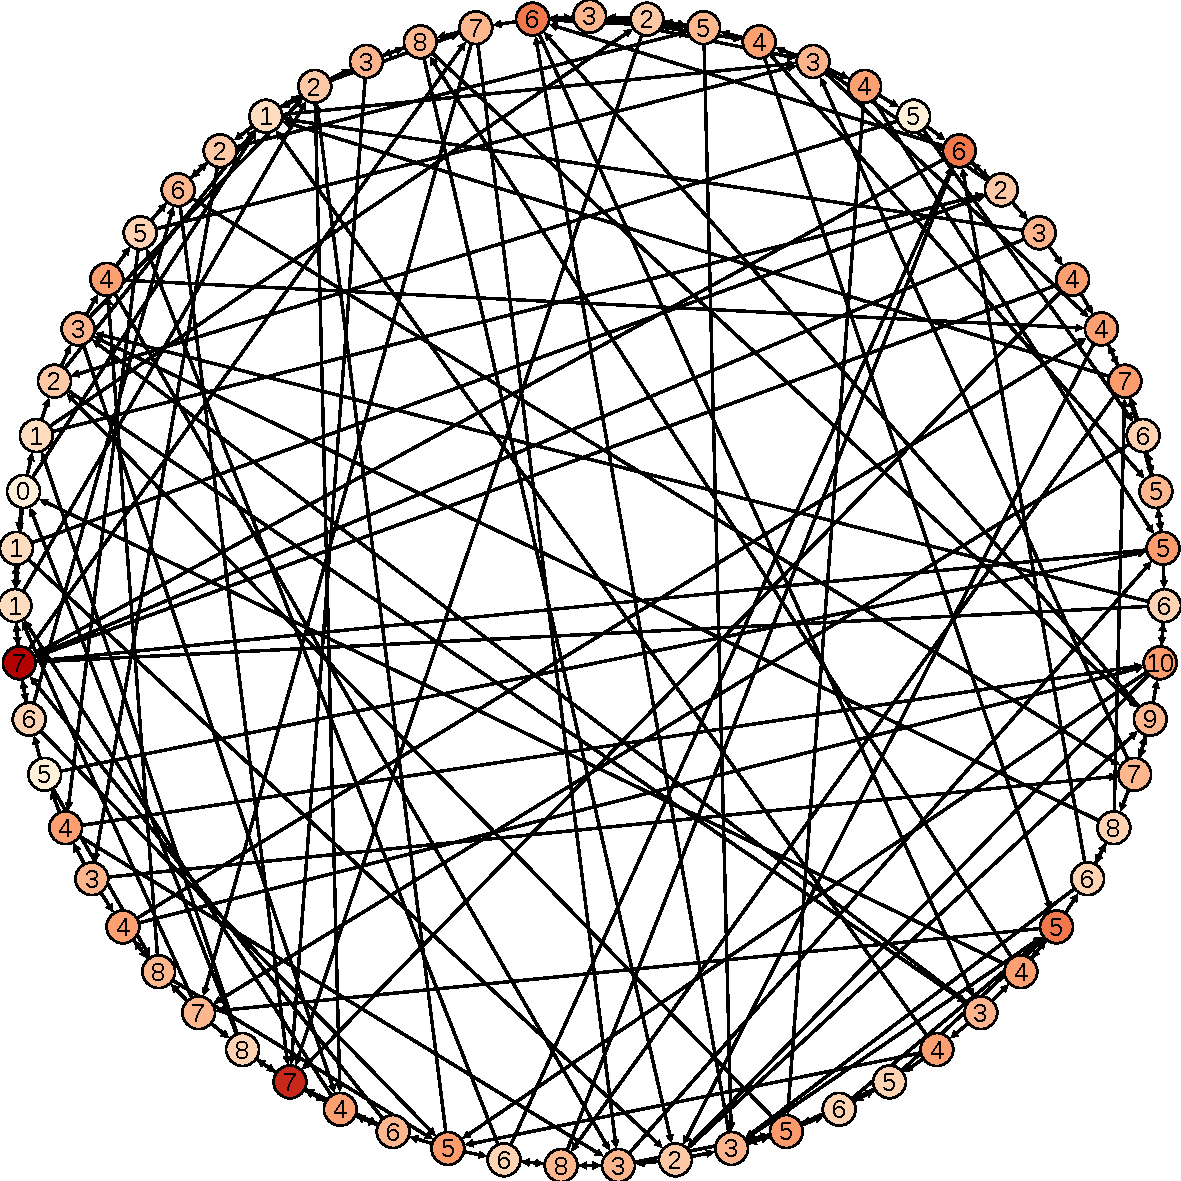
\includegraphics[scale=0.6]{figures/diss_3}
    \caption{Visualization of PolderCast after the end of dissemination}
    \label{fig:diss_2}
    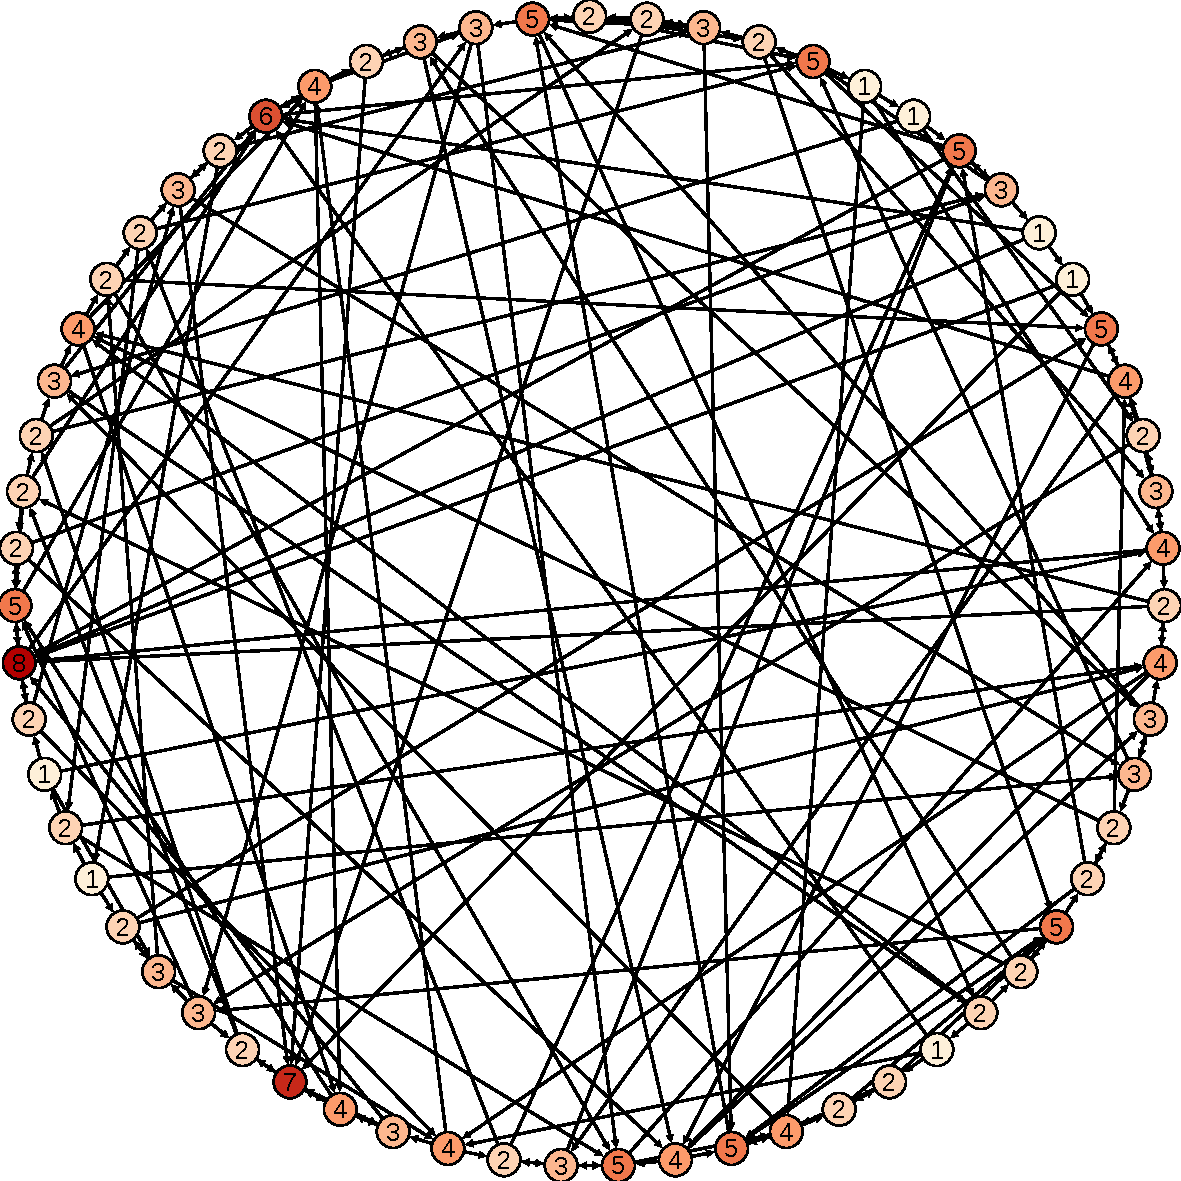
\includegraphics[scale=0.6]{figures/diss_dup_msg}
    \label{fig:dups}
    \caption{Visualization of duplicate publication messages received by
    each node in PolderCast}
\end{figure*}

\subsection{Comparing Pub/Sub Systems Visually}

In Figure~\ref{fig:struct_poldercast} and Figure~\ref{fig:struct_scribe}
we visualize the structure of PolderCast and Scribe respectively. We run
PeerNet experiments in simulation mode, consisting of 1000 nodes, 1000
reporter intervals and 1000 PeerNet cycles. Subscriptions are modeled
after the Twitter dataset found in~\cite{Kwak10www}. The resulting \gexf{} files
are imported into Gephi in order to analyze the overlay structure both
visually as well by calculating certain metrics using the
\emph{Statistics Component}. The calculated values are described in
Table~\ref{tab:struct_metrics}.

\begin{table}[h!]
    \centering
    \begin{tabular}{|l | l | l |}
        \hline
        & PolderCast & Scribe \\ \hline
        \hline
        Number of Nodes & 771 & 771 \\ \hline
        Number of Edges & 24152 & 2700 \\ \hline
        Average Degree & 31.33 & 3.50 \\ \hline
        Graph Diameter & 5 & 15 \\ \hline
        Average Path Length & 2.43 & 5.26 \\ \hline
        Graph Density & 0.041 & 0.005 \\ \hline
        Weakly Connected Components & 7 & 84 \\ \hline
        Strongly Connected Components & 20 & 307 \\ \hline
        Average Clustering Coefficient & 0.249 & 0.035 \\ \hline

    \end{tabular}
    \caption{Metric values for PolderCast and Scribe, calculated using
        the \emph{Statistics Component} in Gephi.}
    \label{tab:struct_metrics}
\end{table}

Inspecting the overlay structure visually enables us to derive certain
information which can guide us in further investigations. For example,
by comparing the overlays, we can observe that the overlay of PolderCast
in Figure~\ref{fig:struct_poldercast} seem to include a lot more edges,
as well as being more dense than the overlay in Scribe, seen in
Figure~\ref{fig:struct_scribe}. Although both overlays consists of the
same number of nodes, PolderCast has almost 10 times the number of edges. This should mean PolderCast also
has a much higher average degree as well as a higher graph density.
Running these metrics reveal that PolderCast indeed have a much higher
degree, almost ten times higher than Scribe. The graph density is also much
higher in PolderCast. Graph density is measured as how far away the graph is
to being complete, where 1 is a complete graph. The low density of Scribe might
be due several nodes being connected at the underlying DHT.\ These edges
are not included in the visualization, but neither are the edges in the
CYCLON or VICINITY modules of PolderCast. Therefore, it is unlikely
that the differences we see in terms of number of edges or density would be much
different if these were included.

The fact that the number of edges in PolderCast is much higher, also
means the overlay is better connected. This is evident if we look at the
number of connected components. Strongly connected components have a
directed path between every pair of nodes, while weakly connected
components are connected through undirected edges. As seen in
Table~\ref{tab:struct_metrics}, the Scribe overlay is more partitioned,
as it includes a higher number of graph components, both strongly
connected as well as weakly connected. The higher number of graph
components in Scribe is likely due to the topics being organized into
separate dissemination trees, where the paths between the rendezvous
nodes are connected at the DHT layer. Also, disconnected nodes are
caused by subscribers not having any topic neighbors online due to
churn.

Using the capabilities of \demo{}, we are also able to look further into
the issue of load balancing. Figure~\ref{fig:polder_in_degree} and
Figure~\ref{fig:scribe_in_degree} visualize the degree of the nodes
in the overlay by color. The deeper red the color of the node is, the
higher its degree. This is useful for spotting potential bottlenecks in
the system in system, as well as getting a general overview of the
degree distribution.

\begin{figure}
    \vspace{-100pt}
    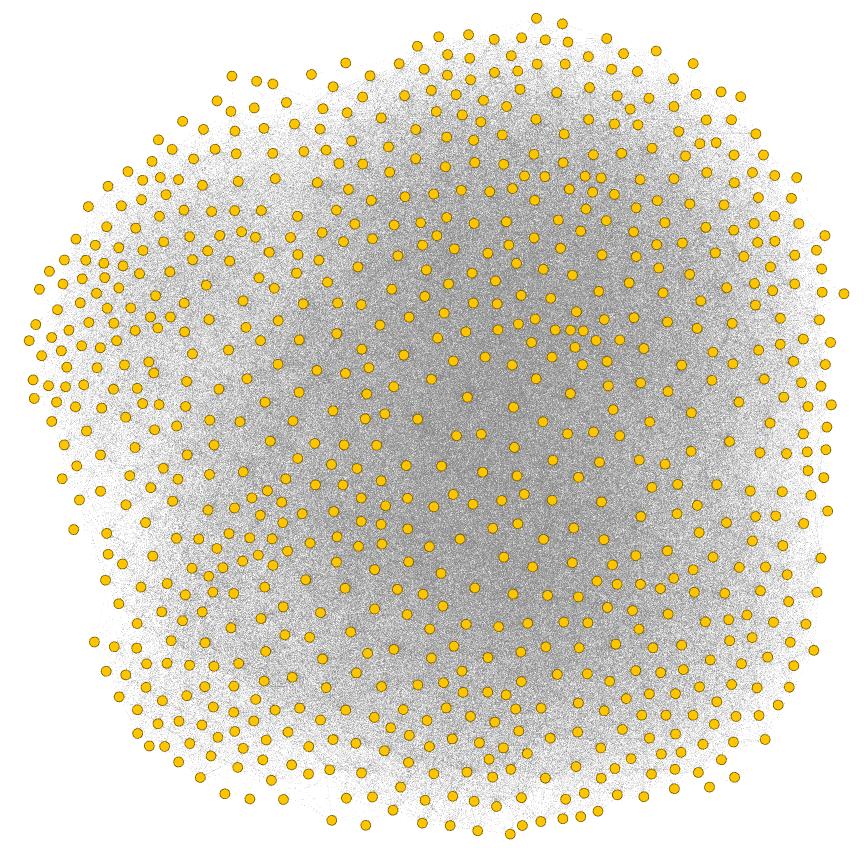
\includegraphics[scale=0.45]{figures/polder_struct}
    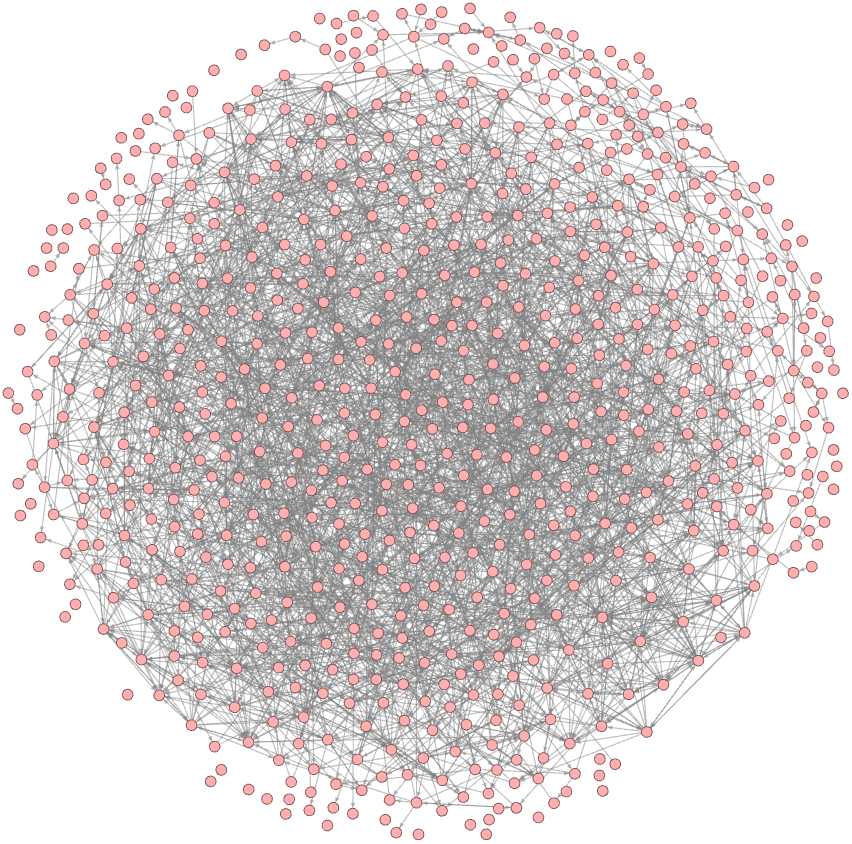
\includegraphics[scale=0.45]{figures/scribe_struct}
    \caption{From top to bottom: Visualizaton of the \textbf{overlay
            strucure} of PolderCast and Scribe}
    \label{fig:struct}
\end{figure}

\begin{figure}
    \vspace{-100pt}
    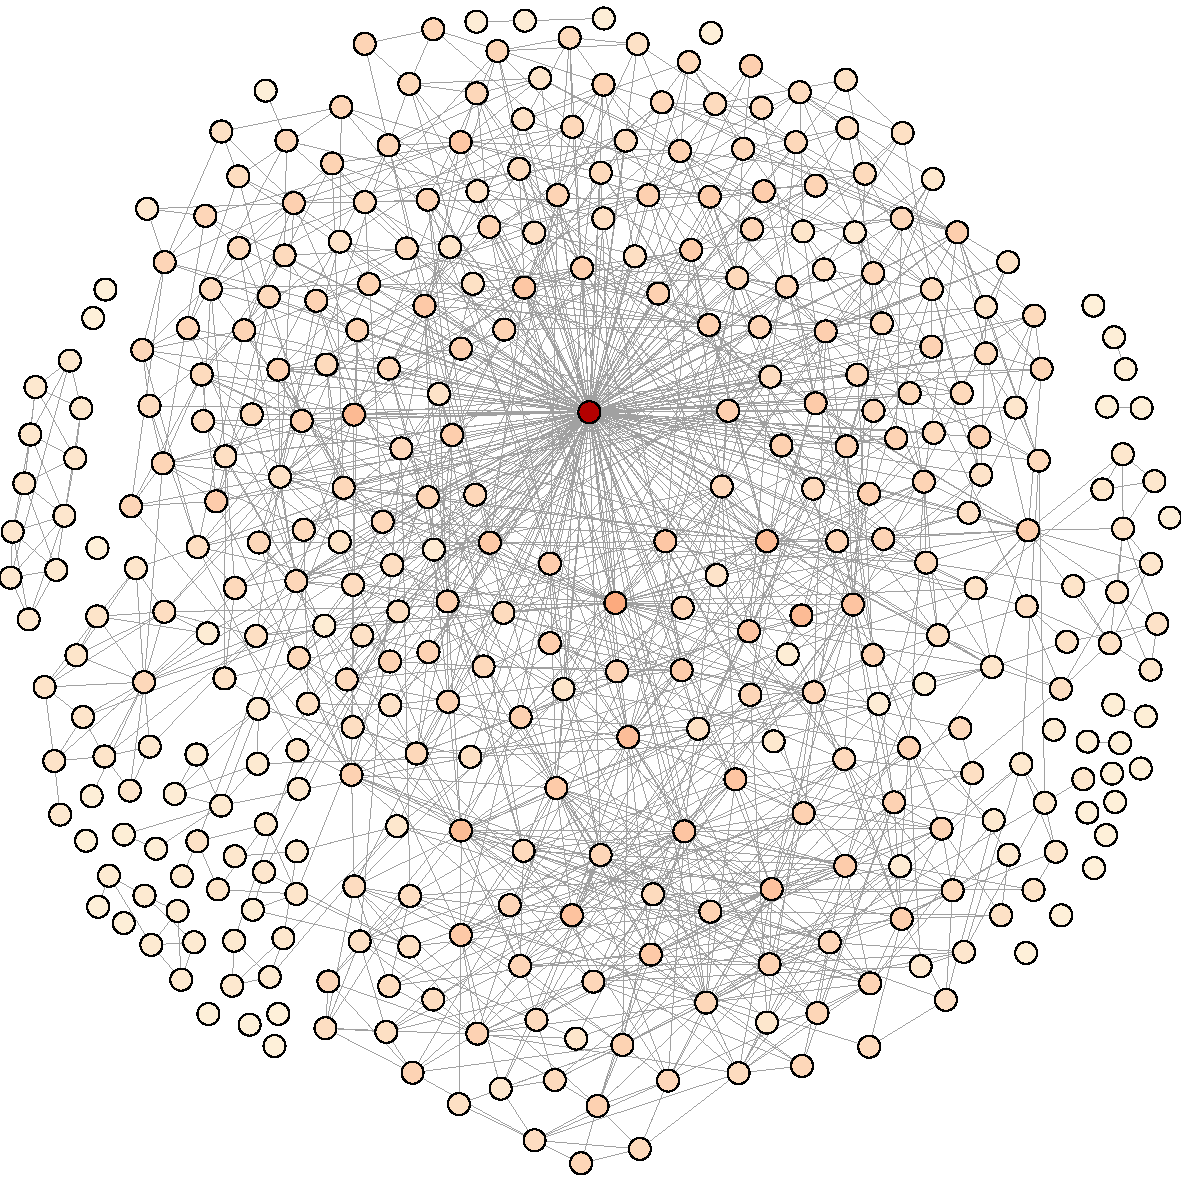
\includegraphics[scale=0.5]{figures/polder_degree}
    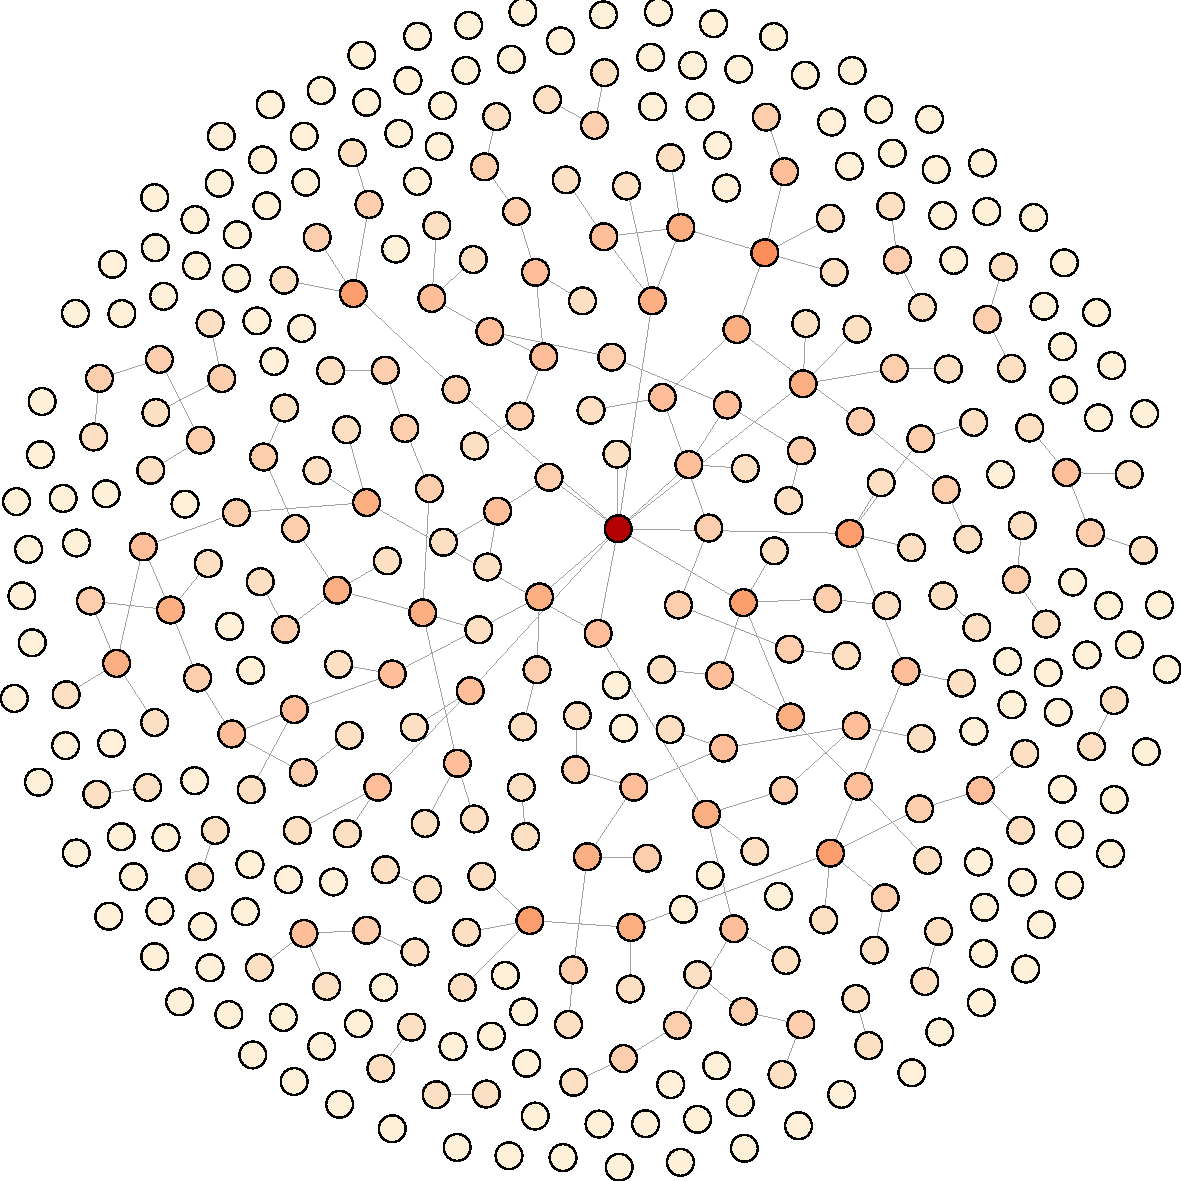
\includegraphics[scale=0.5]{figures/scribe_degree}
    \caption{From top to bottom: Visualization of \textbf{degree} in
        PolderCast and Scribe}
    \label{fig:degree}
\end{figure}

\section{\demo as a Framework for Evaluating Pub/Sub Systems}
\label{sec:viz_eval}

In addition to outputting a \gexf file which can be used to produce
visualizations in Gephi, The collector is also able to generate \csv
files which can be used to plot a time series of metrics such as degree,
clustering coefficient and centralities. Each time point in the time
series will represent a \emph{Reporter Interval}. Although the Data
Laboratory component in Gephi is able to output such \csv files, it is
much more convenient to output them directly from the Collector, as
opening the Gephi GUI-client for the sole purpose of producing such
files manually is more time consuming, especially on older hardware, or
machines without a dedicated graphics card. The Collector is able to do
this trough the Gephi Toolkit, which provides an API for the major
components of Gephi. Which overlay properties to
output is configurable in the Collector.  Currently, the supported
metrics that can be exported to \csv files by the Collector include:

\begin{itemize}
    \item Undirected Degree
    \item In-Degree
    \item Out-Degree
    \item Clustering Coefficient
    \item Betweenness Centrality
    \item Closeness Centrality
    \item Eccentricity Centrality
    \item Topic Diameter
    \item Size of Network
\end{itemize}

This grants researchers and developers of pub/sub protocols who wish to evaluate
the system in question immediate access to several metrics. They do not need to
reimplement algorithms for the metric calculations themselves. All that is
required is to implement the \emph{reporter interface} described in
Section~\ref{sec:arch}. In Chapter~\ref{ch:evaluation} we use this capability of \demo in
order to evaluate PolderCast and Scribe on a set of topology metrics.

\section{Implementation Work}

During our implementation work, we encountered several scenarios were
\demo proved its usefulness as a tool for both developing and debugging
pub/sub protocols. In this section, we will describe some of these
experiences, as well as experiences with other aspects of software
development and distributed systems research such as using test-driven
development and sharing code with the research community.

\subsection{Using Visualizations to Analyze Datasets}

In section~\ref{sec:overview} we mention how we were able to observe a
disconnected component in the RINGS layer of PolderCast, as seen in
Figure~\ref{fig:pold_disc}, and later confirm this was an artefact of
the workload being used. More specifically, we used the \emph{Node Query
    Tool} in Gephi to ensure these nodes had zero overlapping interest
with any other node in the overlay by inspecting the Topics-attribute of
the visualized nodes. This was the first experience we had with the tool, were it
usability was clearly demonstrated. It speaks to how visualizations are
also able to provide information of the datasets being used. In the
scenario we describe, we used a real-world trace from Twitter~\cite{Kwak10www},
which included 1000 user accounts and their subscriptions. However, the
PeerNet simulation only included 100 nodes for testing purposes. This
leads a biased sample of the trace, which in this case lead to a
disconnected component. Being able to run simulations with fixed
parameters but different datasets, and then inspect the resulting
overlay visually is another aspect of using \demo which should prove
useful for researcher of topic-based pub/sub systems.

\subsection{Debugging Pub/Sub Systems Visually}

\begin{figure}[ht!]
    \centering
    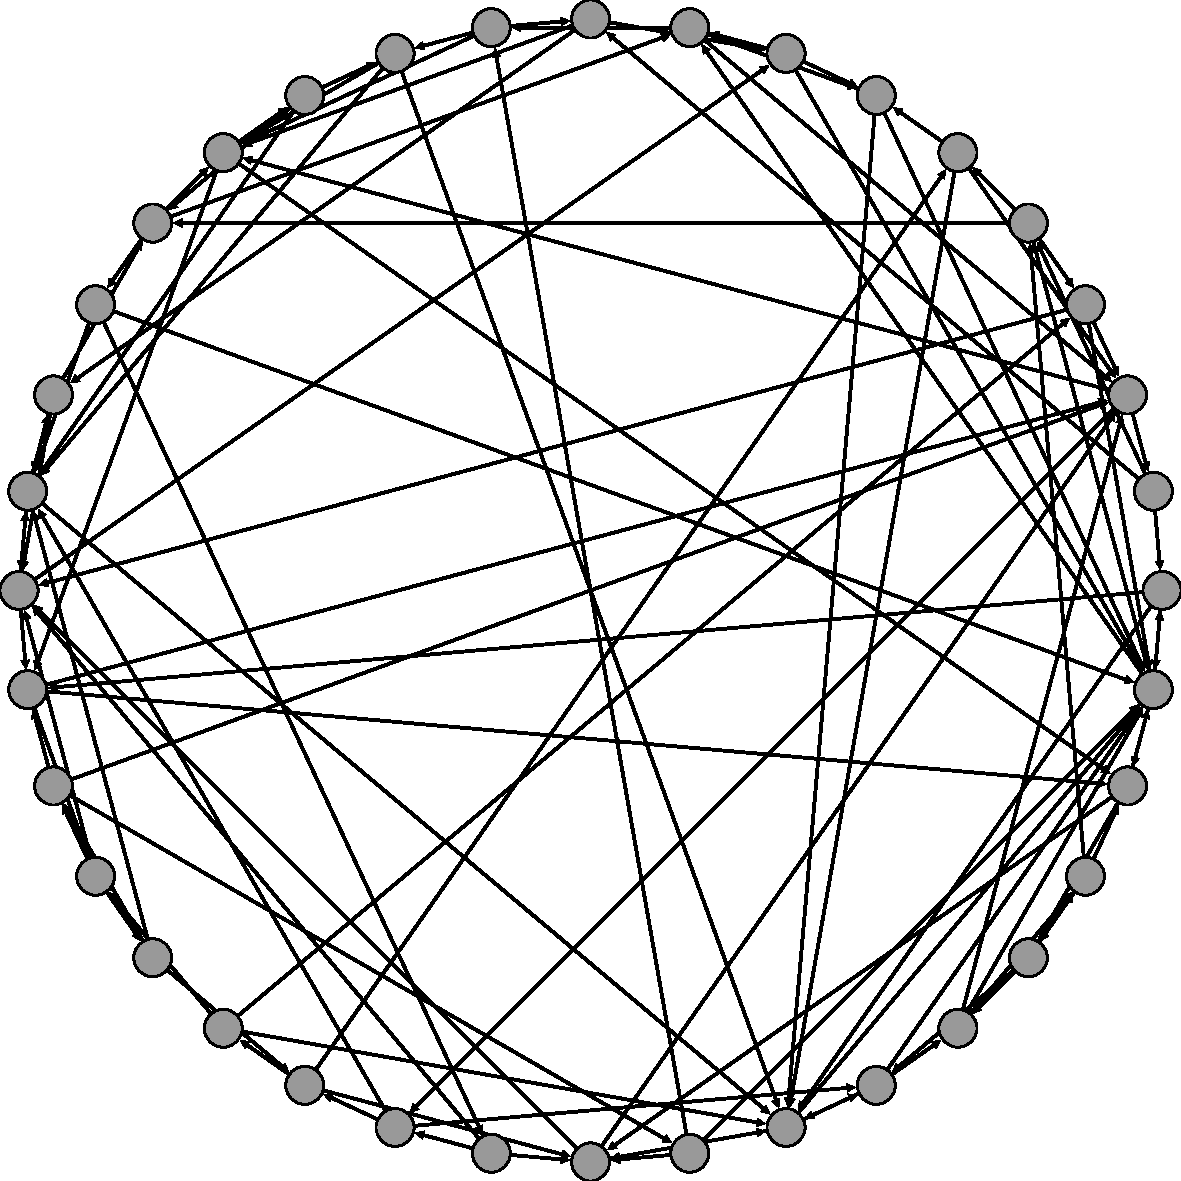
\includegraphics[width=\linewidth]{figures/hitratiobug}
    \caption{Visualization of publication message dissemination in
        PolderCast, which revealed a bug in the implementation of hit-ratio
        calculation}
   \label{fig:hitratiobug}
\end{figure}

When implementing hit-ratio calculation in the Collector, producing a
visualization of the publication message dissemination revealed a bug in the implementation code.
In PolderCast, the hit-ratio in the absence of churn should be 100\%.
However, the Collector would consistently calculate the hit-ratio to
97\%. Usually, the first step in debugging such issues is to isolate the
problem. In this case, there could be a software bug in the
implementation of the pub/sub protocol itself, or the bug might be in
the implementation of the hit-ratio calculation. Using \demo, we were
able to quickly isolate the problem. By producing a visualization of the
publication message dissemination, seen in Figure~\ref{fig:hitratiobug},
we were able to visually confirm that all nodes that took part in the dissemination
received the message. Furthermore, we could confirm this observation by
using the Statistics component in Gephi, which enables calculation of
the number of connected components in the graph.  The calculation
revealed that the graph is a single strongly connected component, i.e.\
from any node in the graph there is a directed path to any other node.
This means that every node received the publication.  However, the
Collector still calculated the hit-ratio to 97\%. This indicates that
the problem is not with the implementation of the protocol, but with the
implementation of the hit-ratio calculation. And indeed, by inspecting
the hit-ratio calculation in the Collector, we revealed a
\emph{off-by-one} software bug, leading to incorrect hit-ratio result.

Debugging is a major part of developing software, and arguably the most
time consuming. And debugging distributed systems is especially hard.
Any tool that aids in debugging is highly valuable to any developer. As
a tool for debugging, \demo{} can aid in both discovering and resolving
bugs, as it provides the developer with instant visual feedback of the
protocol behaviour.


\subsection{Using Test-Driven Development}

Software Development Methodology is an active area of research
which is in part driven by the business needs of the private
sector\cite{janzen2005test}. One popular practice is so-called Test-Driven
Development (TDD). The promoters of TDD claims it increases
productivity and reduces the number of bugs and defects in the
code significantly~\cite{beck2003test}. Research
efforts performed at IBM~\cite{maximilien2003assessing} seems to
lend credibility to these claims. However, the use of TDD is not
prevalent in academia, and in~\cite{janzen2005test} they
recommend further research into the field in order to better
determine its effects.

Using TDD means writing tests before writing any code. There are
different types of test. \emph{unit tests} targets small,
independent pieces of code, typically methods within a single
module or component, while \emph{integration tests} aim to test
code across such modules and components in order to determine
how well they integrate with each other. In our work, we only
took advantage of Unit Tests where suitable using the
JUnit~\cite{junit} and Mockito~\cite{mockito} libraries.
We could also have benefited from a suite of integration tests,
as our implementation is heavily dependent on interoperating
components, as well as file and network IO\@. However, writing
these sort of tests would simply be too time consuming compared
to writing smaller unit tests.

The TDD approach to software development is best described through the
Red-Green-Refactor mantra, which is a central part of the
TDD-philosophy. It can be described through the following steps:

\begin{description}
    \item[Step 1:] Write a test that fails. (Red)
    \item[Step 2:] Make the test pass. (Green)
    \item[Step 3:] Refactor the code while making sure the test
        still passes. (Refactor)
\end{description}

In our experience this routine has been helpful when working
with our implementation code, as it enables us as developer to
refactor with confidence achieving more maintainable code and a
more thoughtful software design. Since we share our
implementation code with the research community by hosting it in
a open repository, any tool or method that helps us improve the
design and maintainability of our project is of great value to
us. Using TDD forced us to think more deeply about what
functionality to implement and how to structure and split the
problem domain into smaller function points. We believe that in
the end, following TDD where its suitable is beneficial to both
programmer productivity as well as programmer happiness. Also,
we are confident that this practice decreased the amount of
technical debt in our project, a problem we find to be commonplace in academia.

\subsection{Sharing Code with the Community}

We believe sharing our code is to the benefit of both \demo{} and the
community. During our presentation at DEBS 2014, the interest in our
tool was high, and we received a fair amount of requests for our
implementation code. Sharing our code by hosting it publicly will
hopefully allow the tool to grow from a prototype into mature product by
allowing anyone to contribute with improvements and bug fixes. It is our
hope that \demo{} will be a lasting contribution to the research
community, and hosting the code publicly is a key part in ensuring the
future of the tool.

\section{Chapter Summary}
